% \makeglossaries
% \sisetup{
% display-per-mode = fraction,
% inline-per-mode = symbol,
% group-separator = {,}
% }

% Acronym definitions
\glsresetall
% \newacronym{mdp}{MDP}{Markov Decision Process}
% \newacronym{pomdp}{POMDP}{Partially Observable Markov Decision Process}
% \newacronym{lstm}{lstm}{long short-term memory}
% \newacronym{dqn}{DQN}{deep Q-network}
% \newacronym{drqn}{DRQN}{deep recurrent Q-network}
% \newacronym{ddqn}{DDQN}{double deep Q-network}
% \newacronym{idm}{IDM}{intelligent driver model}
% \newacronym{rl}{RL}{reinforcement learning}
% \newacronym{ad}{AD}{autonomous driving}
% \newacronym{av}{AV}{autonomous vehicles}
% \newacronym{adas}{ADAS}{advance driver assistance systems}
% \newacronym{mcts}{MCTS}{Monte Carlo tree search}

\def\InputColor{rgb:yellow,5;red,5;white,5}
\def\ConvColor{rgb:yellow,5;red,2.5;white,5}
\def\ConvReluColor{rgb:yellow,5;red,5;white,5}
\def\PoolColor{rgb:red,1;black,0.3}
\def\UnpoolColor{rgb:blue,2;green,1;black,0.3}
\def\FcColor{rgb:blue,5;red,2.5;white,5}
\def\FcReluColor{rgb:blue,5;red,5;white,4}
\def\SoftmaxColor{rgb:magenta,5;black,7}   

\tikzstyle{connection}=[thick,every node/.style={sloped,allow upside down},draw=\edgecolor,opacity=0.7]
\tikzstyle{copyconnection}=[thick,every node/.style={sloped,allow upside down},draw={rgb:blue,4;red,1;green,1;black,3},opacity=0.7]
    
\newcommand{\copymidarrow}{\tikz \draw[-Stealth,line width=0.4mm,draw={rgb:blue,4;red,1;green,1;black,3}] (-0.3,0) -- ++(0.3,0);}


\newcommand{\basenet}[1]{
    % \tikzstyle{connection}=[thick,every node/.style={sloped,allow upside down},draw=\edgecolor,opacity=0.7]
    % \tikzstyle{copyconnection}=[thick,every node/.style={sloped,allow upside down},draw={rgb:blue,4;red,1;green,1;black,3},opacity=0.7]
    
    % \def\BeliefSize{Belief}
    \def\BeliefDepth{#1}
    
    \pic[shift={(0,0,0)}] at (0,0,0) 
        {Box={
            name=input_ego,
            caption= ,
            xlabel={{ , }},
            ylabel= ,
            zlabel=\BeliefSize,
            fill=\InputColor,
            height=2,
            width=1,
            depth=\BeliefDepth
            }
        };
    
    \pic[shift={(1,0,0)}] at (input_ego-east) 
        {Box={
            name=fc_ego,
            caption= FC,
            xlabel={{32, }},
            zlabel=\BeliefSize,
            fill=\FcColor,
            height=2,
            width=2,
            depth=\BeliefDepth
            }
        };
    
    \draw [connection]  (input_ego-east)    -- node {\midarrow} (fc_ego-west);
    % \draw [connection]  (fc_ego-east)    -- node {\midarrow} (flat_ego-west);
    
    \pic[shift={(-0.1,-1.8 ,0)}] at (input_ego-south) 
        {Box={
            name=input_target0,
            caption= ,
            xlabel={{ , }},
            ylabel= ,
            zlabel= ,
            fill=\InputColor,
            height=2,
            width=1,
            depth=\BeliefDepth
            }
        };
    \pic[shift={(-0.1,-0.2,0)}] at (input_target0-south) 
        {Box={
            name=input_target1,
            caption= ,
            xlabel={{ , }},
            ylabel= ,
            zlabel= ,
            fill=\InputColor,
            height=2,
            width=1,
            depth=\BeliefDepth
            }
        };
    
    \pic[shift={(-0.1,-0.2,0)}] at (input_target1-south) 
        {Box={
            name=input_target2,
            caption= ,
            xlabel={{ , }},
            ylabel= ,
            zlabel= ,
            fill=\InputColor,
            height=2,
            width=1,
            depth=\BeliefDepth
            }
        };
    
    \pic[shift={(-0.1,-0.2,0)}] at (input_target2-south) 
        {Box={
            name=input_target3,
            caption= ,
            xlabel={{ , }},
            ylabel= ,
            zlabel=\BeliefSize,
            fill=\InputColor,
            height=2,
            width=1,
            depth=\BeliefDepth
            }
        };
    
    \pic[shift={(1,-0.2,0)}] at (input_target1-east) 
        {Box={
            name=conv0,
            caption= CONV,
            xlabel={{32, }},
            zlabel=\BeliefSize,
            fill=\ConvColor,
            height=8,
            width=2,
            depth=\BeliefDepth
            }
        };
    
    \pic[shift={ (0,0.4,0) }] at (conv0-east) 
        {Box={
            name=stride0,
            caption= ,
            zlabel=stride,
            fill=\PoolColor,
            opacity=0.5,
            height=2,
            width=1,
            depth=\BeliefDepth
            }
        };
    
    \draw [connection]  (input_target1-east)+(0,-2mm)  -- node {\midarrow} (conv0-west)+(0,-1mm);
    % \draw [connection]  (stride0-east)    -- node {\midarrow} (flat_target-west);
    
    \pic[shift={(1,-1.4,0)}] at (fc_ego-east) 
    % \pic[shift={(1.5,1.5,0)}] at (flat_target-east) 
        {Box={
            name=concat,
            caption=CONCAT,
            xlabel={{ , }},
            zlabel= ,
            fill=\UnpoolColor,
            height=16,
            width=2,
            depth=\BeliefDepth
            }
        };
    
    \draw [connection]  (fc_ego-east)    -- node {\midarrow} (concat-west);
    \draw [connection]  (stride0-east)    -- node {\midarrow} (concat-west);
    
    \pic[shift={(.8,0,0)}] at (concat-east) 
        {Box={
            name=fc1,
            caption=FC,
            xlabel={{32, }},
            zlabel=\BeliefSize,
            fill=\FcColor,
            height=8,
            width=2,
            depth=\BeliefDepth
            }
        };
    
    
    \pic[shift={(.8,0,0)}] at (fc1-east) 
        {Box={
            name=fc2,
            caption=FC,
            xlabel={{32, 32}},
            zlabel=\BeliefSize,
            fill=\FcReluColor,
            height=8,
            width=2,
            depth=\BeliefDepth
            }
        };
    
    \draw [connection]  (fc1-east)    -- node {\midarrow} (fc2-west);
    \draw [connection]  (concat-east)    -- node {\midarrow} (fc1-west);
    
}

\newcommand{\baseinput}[1]{
    
    
    % \def\BeliefSize{Belief}
    \def\BeliefDepth{#1}
    
    \pic[shift={(0,0,0)}] at (0,0,0) 
        {Box={
            name=input_ego,
            caption= ,
            xlabel={{ , }},
            ylabel= ,
            zlabel=\BeliefSize,
            fill=\InputColor,
            height=2,
            width=1,
            depth=\BeliefDepth
            }
        };
    
    \pic[shift={(-0.1,-1.0 ,0)}] at (input_ego-south) 
        {Box={
            name=input_target0,
            caption= ,
            xlabel={{ , }},
            ylabel= ,
            zlabel= ,
            fill=\InputColor,
            height=2,
            width=1,
            depth=\BeliefDepth
            }
        };
    \pic[shift={(-0.1,-0.2,0)}] at (input_target0-south) 
        {Box={
            name=input_target1,
            caption= ,
            xlabel={{ , }},
            ylabel= ,
            zlabel= ,
            fill=\InputColor,
            height=2,
            width=1,
            depth=\BeliefDepth
            }
        };
    
    \pic[shift={(-0.1,-0.2,0)}] at (input_target1-south) 
        {Box={
            name=input_target2,
            caption= ,
            xlabel={{ , }},
            ylabel= ,
            zlabel= ,
            fill=\InputColor,
            height=2,
            width=1,
            depth=\BeliefDepth
            }
        };
    
    \pic[shift={(-0.1,-0.2,0)}] at (input_target2-south) 
        {Box={
            name=input_target3,
            caption= ,
            xlabel={{ , }},
            ylabel= ,
            zlabel=\BeliefSize,
            fill=\InputColor,
            height=2,
            width=1,
            depth=\BeliefDepth
            }
        };
}

\newcommand{\makepointcloud}{
    \node[circle, draw=black, minimum size=\radius cm, label=below:{PF}] (pf) at (\pfx, \pfy) {}; 
    \foreach \i in {1,...,15}
    {
        \draw[red, fill=red] (\pfx + rand*0.3 , \pfy + rand*0.3) circle (0.05);
    }
}

%%%%%%%%%%%%%%%%%%%%%%%%%%%%%%%%%%%%%%%%%%%%%%%%%%%%%%%%%%%%%%%%%%%%%%%%%%%%%%%%
\begin{abstract}
This paper investigates different approaches to find a safe and efficient driving strategy through an intersection with other drivers.
Because the intentions of the other drivers to yield, stop, or go are not observable, we use a particle filter to maintain a belief state. 
We study how a reinforcement learning agent can use these representations efficiently during training and evaluation.
This paper shows that an agent trained without any consideration of the intentions of others is both slower at reaching the goal and results in more collisions.
Four algorithms that use a belief state generated by a particle filter are compared. Two of the algorithms have access to the intention only during training while the others do not. The results show that explicitly trying to predict the intention gave the best performance in terms of safety and efficiency.

\end{abstract}

\section{Introduction}
Advancements in \gls{av} technology is expected to create a paradigm shift in how we transport ourselves in the near future and even where we choose to live~\cite{McKinsey2023}. However, one of the major concerns is how to tackle the high social demand for traffic safety under various conditions and scenarios. 
Replacing the human driver with a computer to make all tactical and operational decisions is a difficult task to design. In particular, decision-making in scenarios that require interaction with other road participants, as summarized in a review paper~\cite{Schwarting2018}.

In recent years, decision-making for \gls{av}s in structured scenarios like intersections has attracted a lot of attention in the research society and the automotive industry. A skilled engineer can sometimes solve the decision-making problem for structured traffic scenarios using rule-based methods, e.g., ~\cite{Fletcher2008} and \cite{darpa2008}. Rule-based decision-making is commonly implemented using hierarchical state machines to switch between predefined behaviors, as shown in \cite{Fletcher2008}. However, it can be difficult for an engineer to anticipate every situation and design a suitable strategy that can solve all of them, in particular when drivers are not following the law~\cite{Althoff2021}, and statistics from the Insurance Institute for Highway Safety estimated in \num{2019} that \num{143000} people in the US were injured in red light running crashes and \num{846} of them were killed~\cite{IIHS2019}. 
% These accidents were mainly caused by driver inattention or reckless driving. 
Hence, decision-making for \gls{av}s cannot only rely on traffic rules to be safe, but they also need to be prepared when other traffic participants do not follow them. Furthermore, rule-based approaches has difficulty generalizing to unknown situations and deal with uncertainties, such as the uncertainty of whether other traffic participants intend to follow the rules or not.

In order to handle the uncertainty of predicting other traffic participants' behaviors or intentions, the literature formulates the problem of driving under uncertainty as a \gls{pomdp}, e.g., with intentions as a non-observable state. \gls{pomdp}s can be solved by simulating all possible future motions given different potential behaviors and/or intentions~\cite{Hubmann2017, Sunberg2017}, e.g. \gls{mcts}. Unfortunately, \gls{mcts} requires extensive online computation and can be hard to scale in complex traffic situations with an increasing number of traffic participants, especially when a participant's actions are interdependent on all other participants’ actions. 
Learning-based approaches, like \gls{rl}~\cite{Sutton2018, Isele2018}, can help relieve the burden of designing hand-crafted solutions for all possible scenarios and \Gls{drqn} approaches, \cite{HausknechtS15drqn, zhu2018improving}, showed some promise solving \gls{pomdp} with non-observable states by leveraging past observations or actions. %\gls{mcts} was even combined with \gls{rl} to move the extensive computation from online to offline~\cite{Hoel2018}.
One such approach was proposed in our previous work~\cite{Tram2018}, where a decision-making policy that identifies and chooses a gap in-between cars in an intersection scenario by using a deep Q-learning~\cite{Mnih2013} method and an \gls{lstm} network architecture~\cite{lstm1997}.
The results showed that the policy solved the decision-making problem up to $97\%$ of the time under perfect sensing conditions. The few cases where the \gls{av} ended up in collisions occurred when the \gls{av} and another vehicle had the same velocity and the same distance to the intersection, i.e., the policy had difficulties sorting out the situation because the estimation of the hidden state (intention) was embedded in the neural network architecture. The prediction of surrounding vehicles was especially difficult for low velocities. 

To explicitly estimate the intention of other drivers is not an easy task~\cite{Amsalu2017}. 
\citet{Liebner2012} proposed to estimate driver behavior using a driver model, the so-called \gls{idm} \cite{idm2000}, to infer driver intent in urban intersections, and \citet{Hoermann2017} used a particle filter to estimate the parameters of the \gls{idm}, both works showed promising results when evaluated on real-world data. 
Another approach to estimating the intention is to introduce belief states to capture uncertainties in the environment~\cite{Bouton2017}. The belief state can be used to model the probability distribution over the uncertain world states, e.g., the intention of other road users. \Citet{wang2023} decoupled the belief state modeling (via unsupervised learning) from policy optimization (via \gls{rl}) and claimed that having full observability at learning time, combined with knowing what will not be observable at deployment time, enables an \gls{rl} agent to learn a policy that is more robust to its unobservable states. Another approach using full observability at learning time is QMDP~\cite{Littman1995}, where a model is first trained on the full state space, including the unobservable states, and later evaluated the model on the belief state. Training on full observability can only be done when the unobservable state can be obtained, e.g., using ground truth data and labeling.

% \begin{figure}[!t]
%     \centering
%         \input{YourThesis/papers/belief/tikz/algorithms_list}
%         \caption{This figure illustrates the four different \discuss{considered} in this paper, where the red dots represent the distribution of the particles, $G$ a state estimator, $f$ and $F$ are neural networks with either traditional weights $\theta$ or weights $\theta_\mathrm{GT}$ trained on ground truth. \discuss{This figure is no longer referred to, should we remove it or add a sentence to give an overview of the algorithms?}
%         }
%         \label{fig:algorithms_intro}
% \end{figure}

In this paper, we propose a decoupled approach, similar to \cite{wang2023}, but model the belief state using a particle filter that is tailor-made for the intersection and use the \gls{idm} to model the possible behavior of different intentions similar to \cite{Liebner2012} and \cite{Hoermann2017}. The policy optimization uses the deep Q-learning approach from \cite{Tram2018}, but without the \gls{lstm} layer.
More specifically, we introduce two novel approaches that are safer than their respective baseline by maintaining a belief state using a particle filter and estimating the unobservable states from the belief state before feeding it to the \gls{dqn}, which gives the final action. 
The first approach uses the probability distribution of the intention as input to the \gls{dqn} and the second approach uses a likelihood estimate with a threshold value for the intention decision to make an estimate of the intention before feeding it to the \gls{dqn}.
The proposed approaches are compared with a naive approach that trains on the entire belief state, a standard approximation method from the literature, QMDP~\cite{Littman1995}, and a \gls{dqn} with full observability. The latter approach represents an upper bound of what a \gls{dqn} is capable of if it has perfect sensing and is referred to as the Oracle \gls{dqn}. 

The main contributions of this paper are: 
\begin{itemize}
    \item A decoupled approach that separates belief state modeling, using a particle filter, and policy optimization, using deep Q-learning; 
    \item a tailor-made particle filter implementation with a separate transition model for each intention state;
    %\item Propose two approaches for representing the belief state in a \gls{dqn}. A probability distribution, QID, and a maximum likelihood estimate of the intention, QIE.
    \item representing the intention state as a probability distribution and two approaches for using the distribution in \gls{dqn}.   
    % \item the introduction of two approaches for representing the belief state in a \gls{dqn}:
    % \begin{itemize}
    %     \item Representing the intention state as a probability distribution. 
    %     \item Train the weights of the \gls{dqn} on full observability and estimate non-observable state with a threshold value during evaluation. 
    % \end{itemize}
    
    % \item A detailed investigation of how to combine particle filter estimation with \gls{rl} algorithms for \gls{av} applications.
    % \item An empirical analysis in simulation of the performance of four belief state \gls{dqn} approaches that explicitly consider the intentions of other traffic participants.
\end{itemize}



\section{Mathematical preliminaries}
\label{sec:background}
% The goal of the ego-vehicle is to make driving decisions through an intersection with crossing traffic, where the intention of the other drivers' in this intersection is unknown. 

This section describes the relevant parts of the \gls{pomdp} framework and the notations used in the problem formulation. It also briefly introduces deep Q-learning, which is used to find the driving policy, and the approximation method QMDP used to handle the unknown intention of the other drivers.
Finally, a driving model that describes the behaviors of other drivers is presented. The driver model is later used on multiple occasions in this paper, both as the transition model of all vehicles in the simulation environment and the prediction model in the particle filter. 
% The specific \gls{pomdp} for this problem is later defined in Section~\ref{sec:pomdp_formulation}.
% This section briefly describes the \gls{pomdp} framework, the approximation method QMDP used to estimate the unknown intention, deep Q-learning used to find the driving policy, and the \gls{idm}.

\subsection{Partially observable Markov decision process}
\label{sec:pomdp}
A \gls{pomdp} is a mathematical framework for modeling sequential decision making problems under uncertainty. It is a generalization of the \gls{mdp} that satisfies the Markov property, which requires that the probability distribution of the next state only depends on the current state and the action taken by the agent, not the history of states. 
% The agent in this case is the ego vehicle. 
A \gls{pomdp} consists of a set of states $\mathcal{S}$, a set of actions $\mathcal{A}$, a transition model $T$, a reward function $R$, a set of observations $\Omega$, an observation model $O$, and a discount factor $\gamma \in [0,1)$. Together they create the tuple $(\mathcal{S},\mathcal{A},T,R,\Omega,O,\gamma)$ that formally defines a \gls{pomdp}~\cite{Kochenderfer2015}. The goal is to find a policy that maximizes the expected return. 


In this paper, we denote the driving policy $\pi$, i.e., the driving decision, which in a \gls{pomdp} is formally defined as a mapping from a belief state to an action, where the action corresponds to the decision. The probability of transitioning to a future state $s^\prime$, given a current state $s \in \mathcal{S}$ and action $a \in \mathcal{A}$, is described by the transition model $T(s^\prime \mid s,a)$, while the reward $r$  for transitioning to the new state $s^\prime$ is given by the reward function $R(s,a)$.
% While in a state $s \in \mathcal{S}$ an agent executes an action $a \in \mathcal{A}$, the probability of transitioning to a future state $s^\prime$ is described by the transition model $T(s^\prime \mid s,a)$ and the reward $r$ is given by the reward function $R(s,a)$. 
Note that, in the \gls{pomdp} framework, the agent only has access to partial information contained in its observation $o$ distributed according to $\Pr(o \mid s', a) = O(o, s', a)$.

To accommodate for the missing information, the agent maintains a belief state. A belief state $b$ is a probability distribution such that 
\begin{equation}
b(s) = \Pr(s \mid o_{1:t})
\label{eq:belief_state}
\end{equation}
is the probability of being in state $s$ at time $t$, given observations $o_{1:t}:=\{o_1,o_2,...,o_t\}$ up to time $t$. 
At each time step $t$, the agent updates its belief using a Bayesian filtering approach given the previous belief and the current observation as follows:
\begin{equation}
    b^\prime(s^\prime) \propto O(o \mid s^\prime, a) \int_{s \in S}T(s^\prime \mid s,a)b(s).
\end{equation}

To evaluate different actions $a$, an action-value function $Q(b, a)$ is used
\begin{equation}
    \begin{split}
        Q (b, a)^\pi = R(b,a) + \\
     \gamma \int_o \max_{a \in \mathcal{A}}\int_s b(s) \int_{s^\prime} O(o \mid s^\prime,a) T(s^\prime \mid s,a) \alpha(s^\prime).
    \end{split}
\end{equation}
The action-value function $Q(b, a)^\pi$ represents the expected discounted accumulated reward received by following policy $\pi$ after taking action $a$ from belief state $b$. The optimal policy $\pi^*$ can be found by maximizing the reward
\begin{equation}
    \pi^*(b) =\argmax_a Q(b, a).
    \label{eq:optimal_policy}
\end{equation}
For real-world problems, finding the optimal policy from a belief state is intractable, especially when the state space is continuous~\cite{Kochenderfer2015}. 
% Finding the optimal policy from a belief state can be hard when the state space is continuous~\cite{Kochenderfer2015}. 
In this case, the belief state can be represented as a collection of particles, which simply are samples from the state space, and an approximation referred to as QMDP can be used:
\begin{equation}
    Q(b, a) \approx \sum_s b(s) Q_{\mathrm{MDP}}(s, a)
    \label{eq:qmdp}
\end{equation}
where $Q_{\mathrm{MDP}}$ is the optimal value function of the \gls{mdp} version of the problem that assumes that the agent has full observability.

While finding the optimal $Q^*(b, a)$, in \eqref{eq:optimal_policy}, may be hard, finding $Q_\mathrm{MDP}(s,a)$ is usually easier. 
When the transition function is explicitly defined and the state space is finite, dynamic programming can be used to compute $Q_\mathrm{MDP}(s, a)$. 
However, the transition function is often only accessible in the form of a generative model (\textit{e.g.} a simulator), and the state space is high-dimensional and continuous. In such settings, deep Q-learning to approximate $Q_{\mathrm{MDP}}(s,a)$ can be used,~\cite{Littman1995}. 

In deep Q-learning, the action-value function is represented by a neural network. The function approximating the optimal value function is given by minimizing the loss function derived from the Bellman equation:
\begin{equation}
    J(\theta) = \mathbb{E}_{s^\prime}[(r + \gamma \max_{a^\prime}Q(s^\prime, a^\prime; \theta) - Q(s, a; \theta))^2]
    \label{eq:dqn-loss}
\end{equation}
where $\theta$ represents the weights of the neural network and $(s, a, r, s')$ is obtained from one simulation step in the environment. 
% The weights are updated through gradient updates. 



\subsection{Behavior model}
\label{sec:driver_model}
The general behavior of surrounding vehicles is modeled using \gls{idm}. Besides describing the behavior of all vehicles, including the ego vehicle, the \gls{idm} is also used in the prediction model of the particle filter. The \gls{idm} models a vehicle $n$'s position and velocity as
\begin{align}
    \dot p_n & = v_n\\
    \dot v_n & = a_{\mathrm{max}}\Big(1-\Big(\frac{v_n}{v^\mathrm{desired}_n}\Big)^\delta-\Big( \frac{d^*(v_n,\Delta v_n)}{d_n}\Big)^2\Big) \label{eq:idm} \\
    & \mathrm{with ~} d^*(v_n, \Delta v_n) = d_0 + v_n T_{\mathrm{gap}} + \frac{v_n \Delta v_n}{2 \sqrt{a_{\mathrm{max}} \alpha_b}} \nonumber
\end{align}
where $v^\mathrm{desired}_n$ is the desired velocity, $d_0$ is the minimum distance between cars, $T_{\mathrm{gap}}$ is the desired time gap to the vehicle in front, $a_\mathrm{max}$ is the maximum vehicle acceleration, $d_n$ is the distance to the vehicle in front, $\Delta v_n = v_n - v_{n-1}$ is the velocity difference between vehicle $n$ and the vehicle directly in front $n-1$, and $\alpha_b$ and $\delta$ are model parameters for comfortable deceleration or acceleration.


The acceleration can be simplified into two terms: an interaction term for when there is a vehicle in front 
\begin{align}
     a^\text{int}_n &=  -a_{max} \Big(\frac{d^*(v_n,\Delta v_n)}{d_n} \Big) ^2  \nonumber \\
     &= -a_{max} \Big(\frac{d_0 + v_n T_{\mathrm{gap}}}{d_n} + \frac{v_n \Delta v_n}{2 \sqrt{a_{\mathrm{max}} \alpha_b} d_n} \Big) ^2
     \label{eq:idm_int}
\end{align}

and free road term, when there is no leading vehicle
\begin{equation}
    a^\text{free}_n= a_\mathrm{max}\Big(1-\Big(\frac{v_n}{v^\mathrm{desired}_n}\Big)^\delta\Big).
    \label{eq:idm_free}
\end{equation}


\section{Proposed approach}
\label{sec:approach}

In this section, the intersection problem is modeled as a POMDP, and the particle filter used to estimate the belief state and its uncertainty is introduced. Finally, we present the \gls{rl} algorithms that are used to train the agent, controlling the ego vehicle.

\subsection{POMDP formulation}
\label{sec:pomdp_formulation}

The problem setting considered in this work is an intersection shown in Figure~\ref{fig:states}, and here we outline a general overview of the \gls{pomdp} formulation, whereas Section~\ref{sec:experiments} specifies the numerical values. 
The ego vehicle approaches an intersection with at least one other vehicle on the perpendicular lane with about the same time-to-intersection assuming they keep a constant velocity. The goal for the ego vehicle is to reach the other side of the intersection as fast as possible without colliding with the other cars. With only onboard sensors on the ego vehicle, it can observe the physical state of other vehicles but not the drivers' intention. 

Such an intersection problem can be described as a \gls{pomdp} with \\ $(\mathcal{S},\mathcal{A},T,R,\Omega,O,\gamma)$ as:

\subsubsection{State space, $\mathcal{S}$}
\begin{figure}[!t]
    \centering
        % 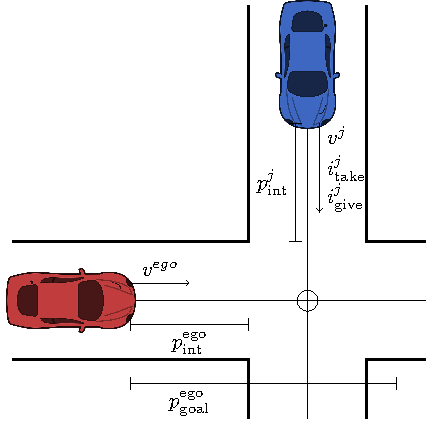
\includegraphics[width=0.6\columnwidth]{figures/figures-observations.pdf}
        % \begin{tikzpicture}
    
%     % Crossing
%     \def\crossverticalx{0}
%     \def\crosstopy{6}
%     \def\crossboty{-2.0}
%     \def\crossleftx{-6}
%     \def\crossrightx{2.0}
%     \def\roadwidth{1.5}
    
%     \draw[thick] (\crossleftx, \roadwidth/2) -- (-\roadwidth/2, \roadwidth/2) -- (-\roadwidth/2, \crosstopy);
%     \draw[thick] (\crossleftx, -\roadwidth/2) -- (-\roadwidth/2, -\roadwidth/2) -- (-\roadwidth/2, \crossboty);
%     \draw[thick] (\roadwidth/2, \crosstopy) -- (\roadwidth/2, \roadwidth/2) -- (\crossrightx, \roadwidth/2);
%     \draw[thick] (\roadwidth/2, \crossboty) -- (\roadwidth/2, -\roadwidth/2) -- (\crossrightx, -\roadwidth/2);
    
%     % cars
%     \node[inner sep=0pt] (ego_car) at (\crossleftx+1,0)
%     {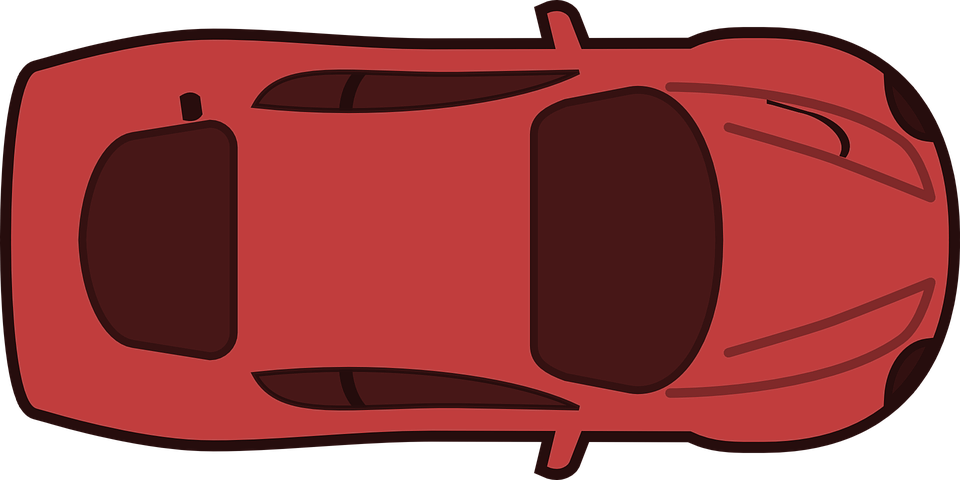
\includegraphics[width=0.10\textwidth, angle=0]{tikz/ego_car_top_down.png}};
%     % \draw (-5, -0.5) rectangle ++(2, 1);
%     \draw[->] ([yshift=0.2cm]ego_car.east) -- node[above] {$v^{ego}$} ($ (ego_car) + (2,0.2)$ );
%     \draw[|-|] ([yshift=-0.2cm]ego_car.east) -- node[below] {$p^{ego}_{0}=v^{ego}*\tau_{int}$} (-\roadwidth/2,-0.2);
%     % \draw (\x, \y) -- node[below] {$p_\mathrm{int}^\mathrm{ego}$} (\xend, \y);
    
%     \node[inner sep=0pt] (target_car_3) at (0,\crosstopy-1)
%     {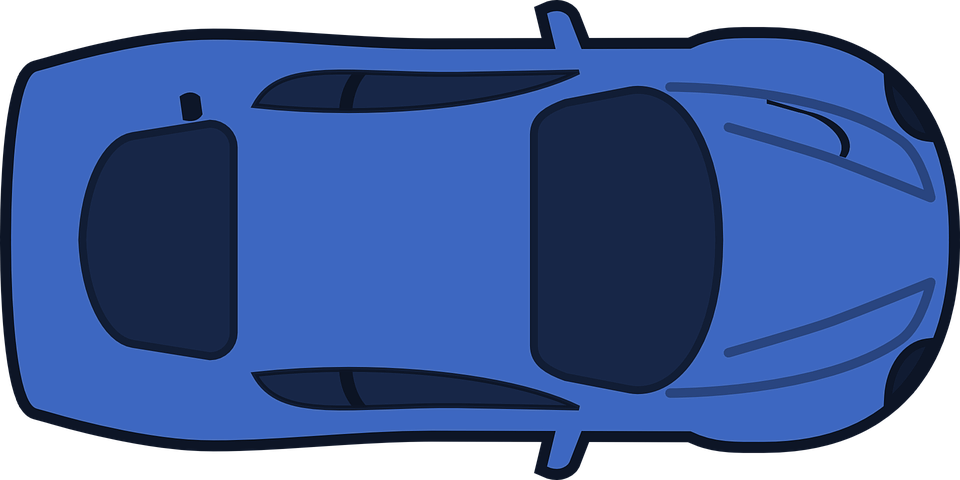
\includegraphics[width=.10\textwidth, angle=-90]{tikz/target_car_top_down.png}};
%     \node (tc_text3a) [right=of target_car_3, align=center, xshift=-0.5cm] {Car 3};
%     \node (tc_text3b) [left=of target_car_3, align=center, xshift=0.5cm] {Conflict Car};
%     \draw[->] ([xshift=0.2cm]target_car_3.south) -- node[right] {$v^{3}_0$} ($ (target_car_3) + (.2,-2)$ );
%     \draw[|-|] ([xshift=-0.5cm]target_car_3.south) -- (-0.5,\roadwidth/2);
%     \node (tc_tti) [below left= 0.2cm and -0.7cm of target_car_3, align=center] {$p^3_{0}$  \\ $\tau_{int}$};
    
%     % \draw (-0.5, 3) rectangle ++(1, 2);
%     \node[inner sep=0pt] (target_car_2) at (0,\roadwidth+0.5)
%     {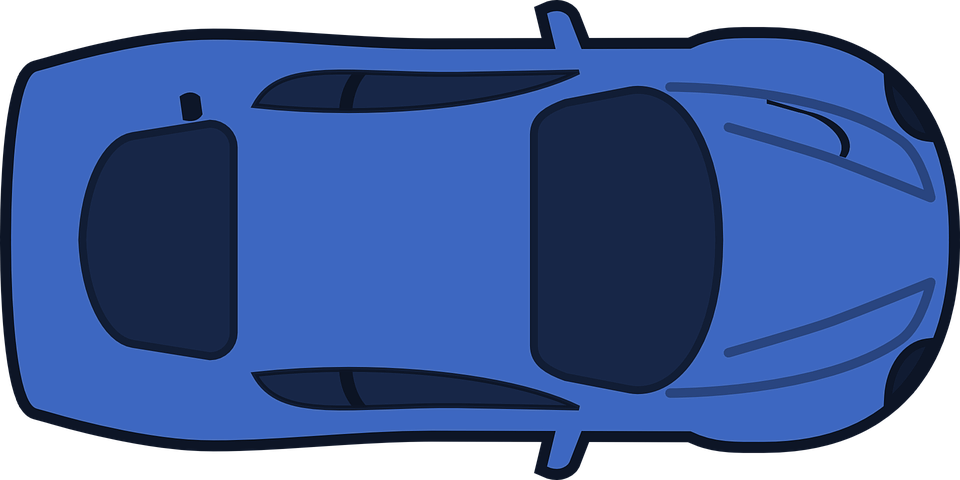
\includegraphics[width=.10\textwidth, angle=-90]{tikz/target_car_top_down.png}};
%     \node (tc_text2) [right=of target_car_2, xshift=-0.5cm] {Car 2};
    
%     \node[inner sep=0pt] (target_car_1) at (0,-\roadwidth+0.5)
%     {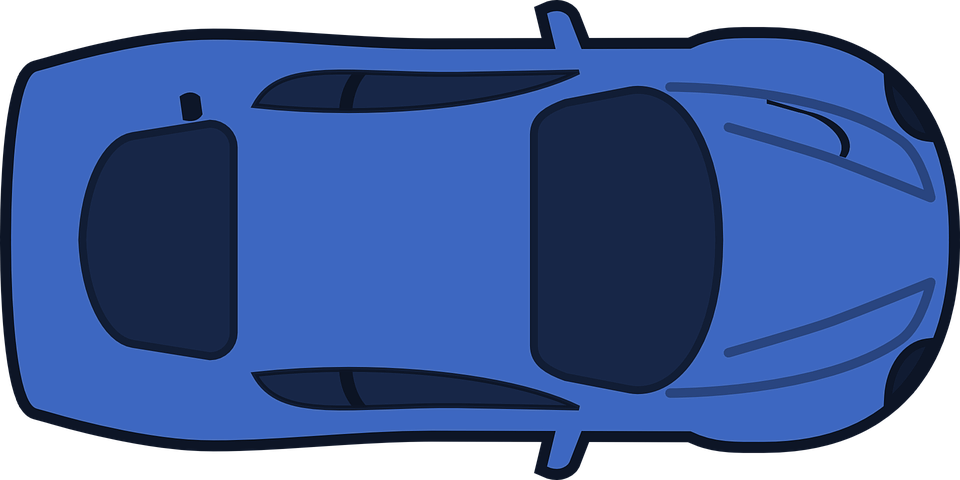
\includegraphics[width=.10\textwidth, angle=-90]{tikz/target_car_top_down.png}};
%     \node (tc_text1) [right=of target_car_1, xshift=-0.5cm] {Car 1};
    
% \end{tikzpicture}

\begin{tikzpicture}

% Crossing
\def\addjust{-1}
\draw[thick] (-5-\addjust, .5) -- (-0.6, 0.6) -- (-.6, 4.2+\addjust);
\draw[thick] (-5-\addjust, -.6) -- (-.6, -.6) -- (-.6, -2.2);
\draw[thick] (.6, 4.2+\addjust) -- (.6, .6) -- (2, .6);
\draw[thick] (.6, -2.2) -- (.6, -.6) -- (2, -.6);

\draw (-3, 0) -- (2, 0);
\draw (0, 3) -- (0, -2);

% cars
\node[inner sep=0pt] (ego_car) at (-4-\addjust,0)
{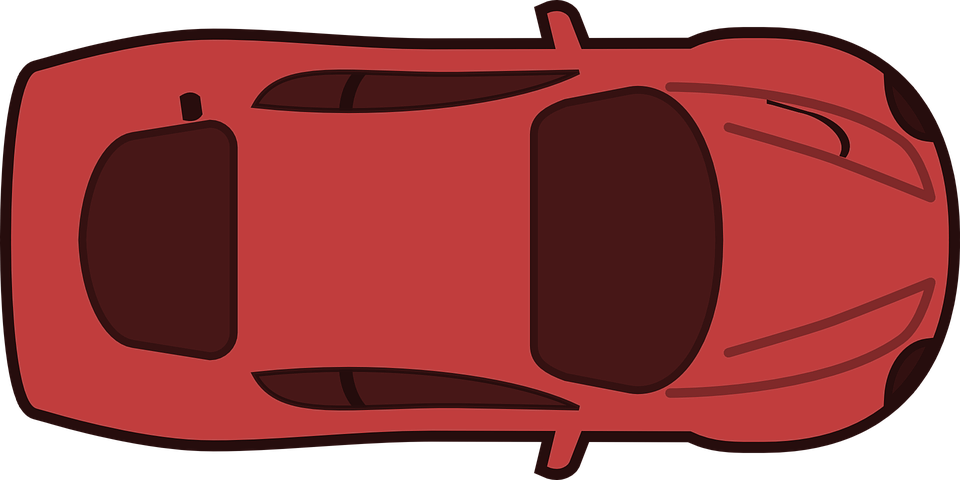
\includegraphics[width=.08\textwidth, angle=0]{tikz/ego_car_top_down.png}};
%		\draw (-5, -0.5) rectangle ++(2, 1);
\node[inner sep=0pt] (target_car1) at (0,3.6+\addjust) {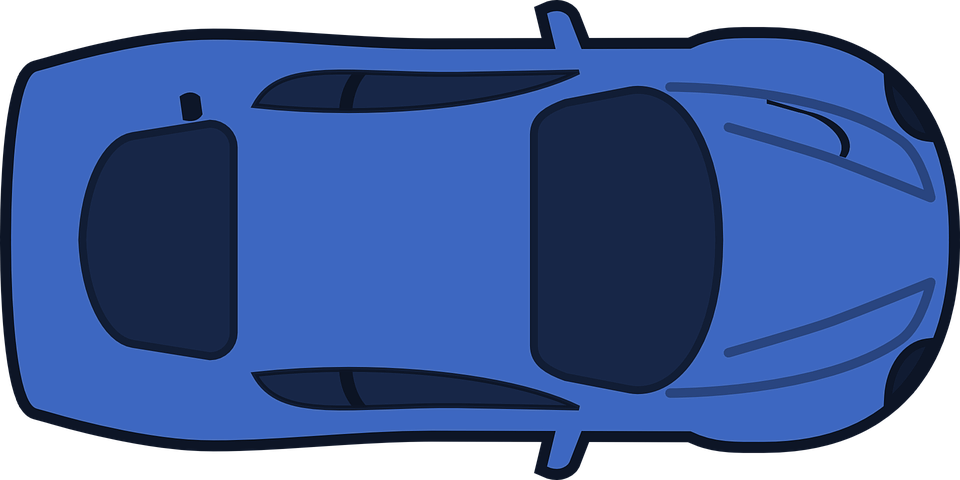
\includegraphics[width=.08\textwidth, angle=-90]{tikz/target_car_top_down.png}};
%		\draw (-0.5, 3) rectangle ++(1, 2);
\node[inner sep=0pt] (target_car2) at (0,\addjust-.3) {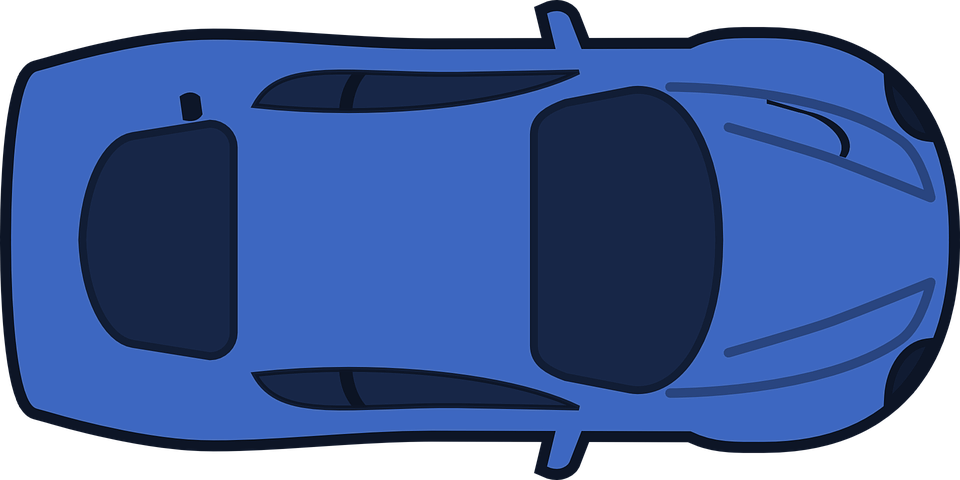
\includegraphics[width=.08\textwidth, angle=-90]{tikz/target_car_top_down.png}};


\draw[->] (-3.3-\addjust, 0.1) -- node[above] {$v_{ego}$} (-1.9-\addjust, 0.1);
\def\x{0.1}
\draw[->] (\x, 3+\addjust) -- (\x, 1.0);

\draw (\x, 2.8+\addjust) node[right] {$v_{n}$} (\x, 2.5+\addjust) 
    -- node[right] {$\zeta_{n}$} (\x, 2+\addjust);
    % -- node[right] {$i^{j}$} (\x, 1.5);
%		\draw[->] (-3, -0.3) -- node[below] {$a_{ego}$} (-2, -0.3);

% Disatance
\draw (0,0) circle (5pt);
% \node at (1.2, -0.3) {crossing point};

% \def\x{-1}
% \def\y{-2}
% \draw (\x, \y) -- node[below] {$\delta^e$} (0, \y); 
% \draw (\x, \y+0.1) -- (\x, \y-0.1);
\def\x{-3}
\def\xend{-.6}
\def\y{-0.08}
\draw (\x, \y) -- node[below] {$p^\mathrm{int}_\mathrm{ego}$} (\xend, \y);
\draw (\x, \y+0.1) -- (\x, \y-0.1);
\draw (\xend, \y+0.1) -- (\xend, \y-0.1);

\def\x{-3}
\def\xend{1.5}
\def\y{-.9}
\draw (\x, \y) -- node[below] {$p^\mathrm{goal}_\mathrm{ego}$} (-1, \y) -- (\xend, \y);
% \draw (-1, \y)-- (\xend, \y);
\draw (\x, \y+0.1) -- (\x, \y-0.1);
\draw (\xend, \y+0.1) -- (\xend, \y-0.1);

\def\x{-0.1}
\def\y{3+\addjust}
\def\yend{.6}
\draw (\x, \y) -- node[left] {$p_{n}$} (\x, \yend);
\draw (\x-0.1, \y) -- (\x+0.1, \y);
\draw (\x-0.1, \yend) -- (\x+0.1, \yend);
%	\def\x{2}
%	\def\y{0}
%	\draw (\x, \y) -- node[right] {$\delta^j$} (\x, 1);
%	\draw (\x-0.1, \y) -- (\x+0.1, \y);

\end{tikzpicture}\\
        \caption{State definitions for the intersection. The red vehicle is the ego vehicle.}
    \label{fig:states}
\end{figure}
% \begin{figure}
%     \centering
%     \begin{subfigure}[b]{0.49\columnwidth}
%         % \begin{tikzpicture}
    
%     % Crossing
%     \def\crossverticalx{0}
%     \def\crosstopy{6}
%     \def\crossboty{-2.0}
%     \def\crossleftx{-6}
%     \def\crossrightx{2.0}
%     \def\roadwidth{1.5}
    
%     \draw[thick] (\crossleftx, \roadwidth/2) -- (-\roadwidth/2, \roadwidth/2) -- (-\roadwidth/2, \crosstopy);
%     \draw[thick] (\crossleftx, -\roadwidth/2) -- (-\roadwidth/2, -\roadwidth/2) -- (-\roadwidth/2, \crossboty);
%     \draw[thick] (\roadwidth/2, \crosstopy) -- (\roadwidth/2, \roadwidth/2) -- (\crossrightx, \roadwidth/2);
%     \draw[thick] (\roadwidth/2, \crossboty) -- (\roadwidth/2, -\roadwidth/2) -- (\crossrightx, -\roadwidth/2);
    
%     % cars
%     \node[inner sep=0pt] (ego_car) at (\crossleftx+1,0)
%     {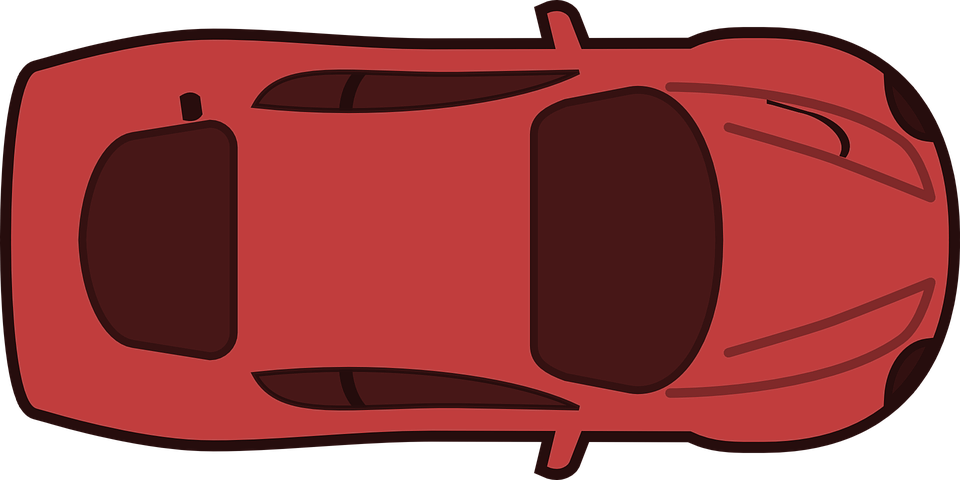
\includegraphics[width=0.10\textwidth, angle=0]{tikz/ego_car_top_down.png}};
%     % \draw (-5, -0.5) rectangle ++(2, 1);
%     \draw[->] ([yshift=0.2cm]ego_car.east) -- node[above] {$v^{ego}$} ($ (ego_car) + (2,0.2)$ );
%     \draw[|-|] ([yshift=-0.2cm]ego_car.east) -- node[below] {$p^{ego}_{0}=v^{ego}*\tau_{int}$} (-\roadwidth/2,-0.2);
%     % \draw (\x, \y) -- node[below] {$p_\mathrm{int}^\mathrm{ego}$} (\xend, \y);
    
%     \node[inner sep=0pt] (target_car_3) at (0,\crosstopy-1)
%     {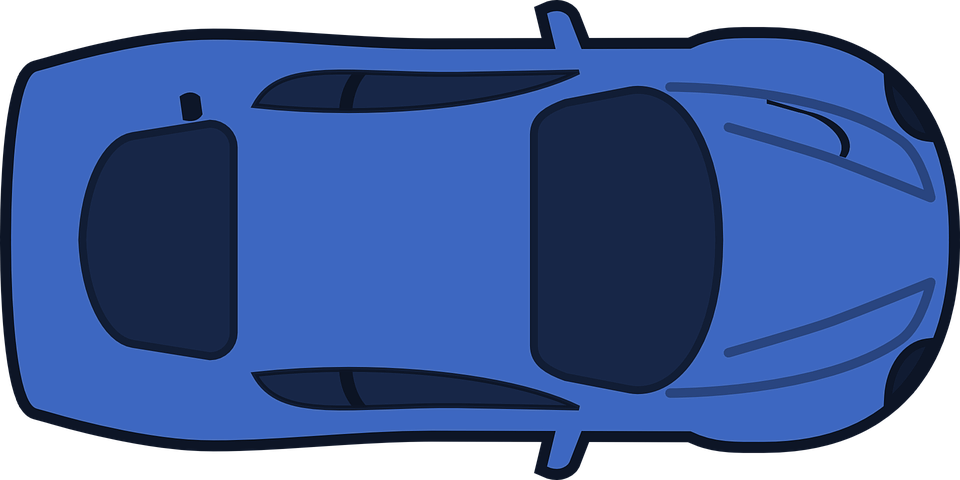
\includegraphics[width=.10\textwidth, angle=-90]{tikz/target_car_top_down.png}};
%     \node (tc_text3a) [right=of target_car_3, align=center, xshift=-0.5cm] {Car 3};
%     \node (tc_text3b) [left=of target_car_3, align=center, xshift=0.5cm] {Conflict Car};
%     \draw[->] ([xshift=0.2cm]target_car_3.south) -- node[right] {$v^{3}_0$} ($ (target_car_3) + (.2,-2)$ );
%     \draw[|-|] ([xshift=-0.5cm]target_car_3.south) -- (-0.5,\roadwidth/2);
%     \node (tc_tti) [below left= 0.2cm and -0.7cm of target_car_3, align=center] {$p^3_{0}$  \\ $\tau_{int}$};
    
%     % \draw (-0.5, 3) rectangle ++(1, 2);
%     \node[inner sep=0pt] (target_car_2) at (0,\roadwidth+0.5)
%     {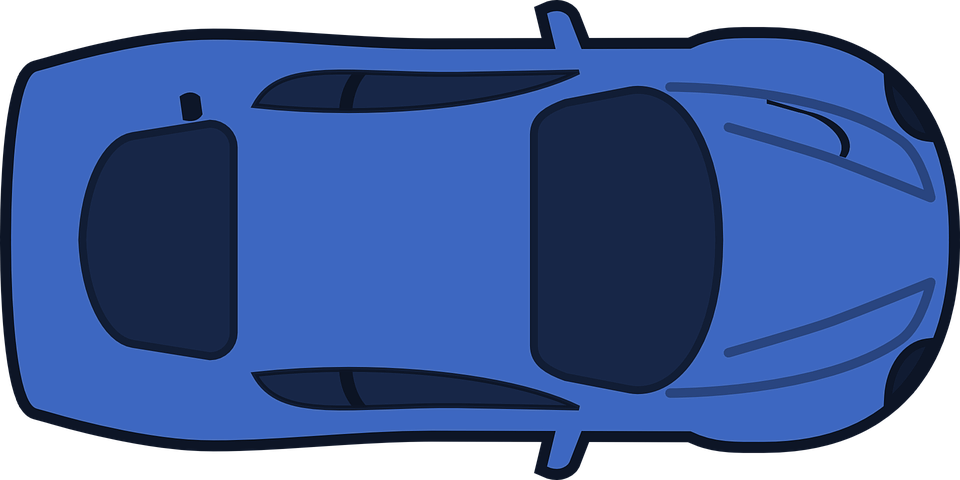
\includegraphics[width=.10\textwidth, angle=-90]{tikz/target_car_top_down.png}};
%     \node (tc_text2) [right=of target_car_2, xshift=-0.5cm] {Car 2};
    
%     \node[inner sep=0pt] (target_car_1) at (0,-\roadwidth+0.5)
%     {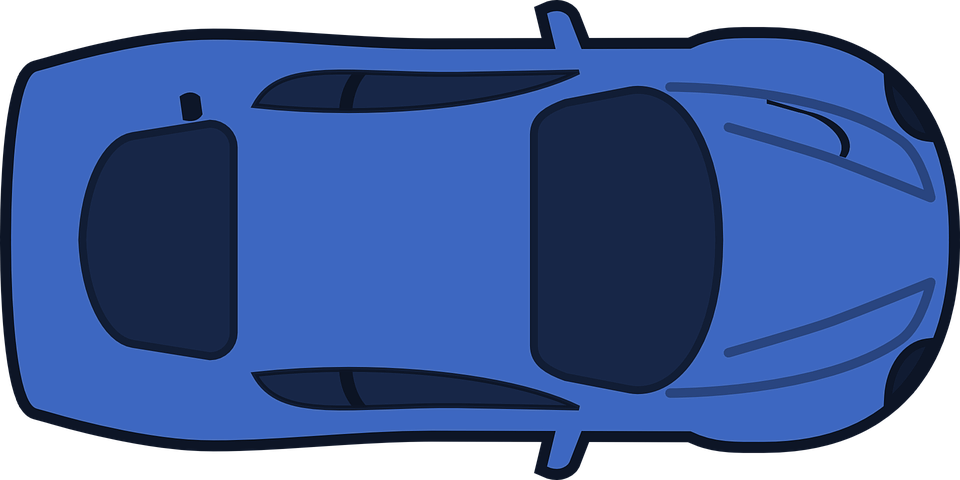
\includegraphics[width=.10\textwidth, angle=-90]{tikz/target_car_top_down.png}};
%     \node (tc_text1) [right=of target_car_1, xshift=-0.5cm] {Car 1};
    
% \end{tikzpicture}

\begin{tikzpicture}

% Crossing
\def\addjust{-1}
\draw[thick] (-5-\addjust, .5) -- (-0.6, 0.6) -- (-.6, 4.2+\addjust);
\draw[thick] (-5-\addjust, -.6) -- (-.6, -.6) -- (-.6, -2.2);
\draw[thick] (.6, 4.2+\addjust) -- (.6, .6) -- (2, .6);
\draw[thick] (.6, -2.2) -- (.6, -.6) -- (2, -.6);

\draw (-3, 0) -- (2, 0);
\draw (0, 3) -- (0, -2);

% cars
\node[inner sep=0pt] (ego_car) at (-4-\addjust,0)
{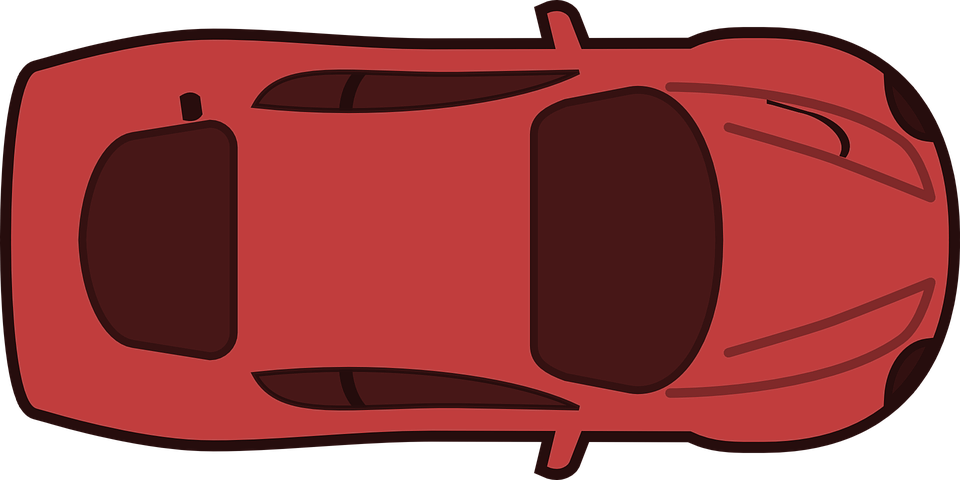
\includegraphics[width=.08\textwidth, angle=0]{tikz/ego_car_top_down.png}};
%		\draw (-5, -0.5) rectangle ++(2, 1);
\node[inner sep=0pt] (target_car1) at (0,3.6+\addjust) {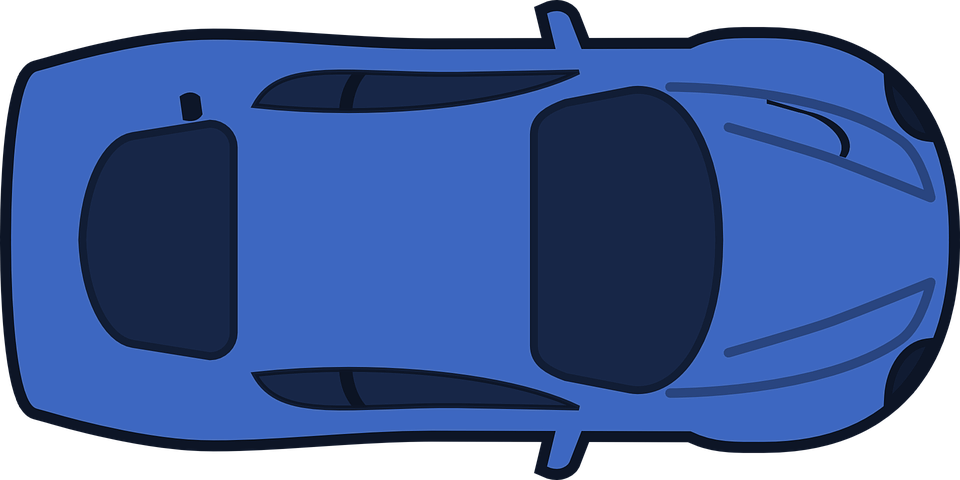
\includegraphics[width=.08\textwidth, angle=-90]{tikz/target_car_top_down.png}};
%		\draw (-0.5, 3) rectangle ++(1, 2);
\node[inner sep=0pt] (target_car2) at (0,\addjust-.3) {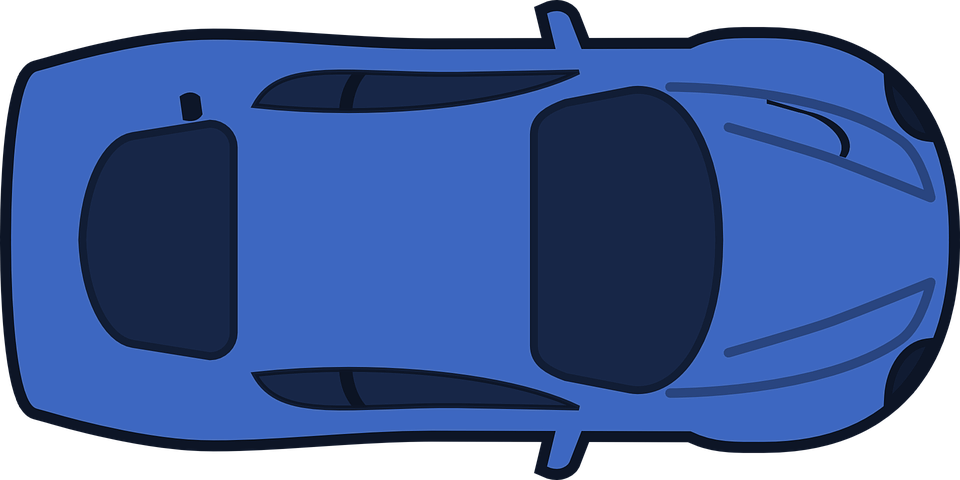
\includegraphics[width=.08\textwidth, angle=-90]{tikz/target_car_top_down.png}};


\draw[->] (-3.3-\addjust, 0.1) -- node[above] {$v_{ego}$} (-1.9-\addjust, 0.1);
\def\x{0.1}
\draw[->] (\x, 3+\addjust) -- (\x, 1.0);

\draw (\x, 2.8+\addjust) node[right] {$v_{n}$} (\x, 2.5+\addjust) 
    -- node[right] {$\zeta_{n}$} (\x, 2+\addjust);
    % -- node[right] {$i^{j}$} (\x, 1.5);
%		\draw[->] (-3, -0.3) -- node[below] {$a_{ego}$} (-2, -0.3);

% Disatance
\draw (0,0) circle (5pt);
% \node at (1.2, -0.3) {crossing point};

% \def\x{-1}
% \def\y{-2}
% \draw (\x, \y) -- node[below] {$\delta^e$} (0, \y); 
% \draw (\x, \y+0.1) -- (\x, \y-0.1);
\def\x{-3}
\def\xend{-.6}
\def\y{-0.08}
\draw (\x, \y) -- node[below] {$p^\mathrm{int}_\mathrm{ego}$} (\xend, \y);
\draw (\x, \y+0.1) -- (\x, \y-0.1);
\draw (\xend, \y+0.1) -- (\xend, \y-0.1);

\def\x{-3}
\def\xend{1.5}
\def\y{-.9}
\draw (\x, \y) -- node[below] {$p^\mathrm{goal}_\mathrm{ego}$} (-1, \y) -- (\xend, \y);
% \draw (-1, \y)-- (\xend, \y);
\draw (\x, \y+0.1) -- (\x, \y-0.1);
\draw (\xend, \y+0.1) -- (\xend, \y-0.1);

\def\x{-0.1}
\def\y{3+\addjust}
\def\yend{.6}
\draw (\x, \y) -- node[left] {$p_{n}$} (\x, \yend);
\draw (\x-0.1, \y) -- (\x+0.1, \y);
\draw (\x-0.1, \yend) -- (\x+0.1, \yend);
%	\def\x{2}
%	\def\y{0}
%	\draw (\x, \y) -- node[right] {$\delta^j$} (\x, 1);
%	\draw (\x-0.1, \y) -- (\x+0.1, \y);

\end{tikzpicture}\\
%         % \caption{State definitions for the intersection. The red vehicle is the ego vehicle.}
%     \end{subfigure}
%     \begin{subfigure}[b]{0.49\columnwidth}
%         \input{YourThesis/papers/belief/tikz/conflict_car_example}
%         % \caption{Initial state of a scenario with three other cars and ego car initial position $p^0_\mathrm{ego}$ is set to have the same time to intersection $\tau_{tti}$ as the conflict car, $p_\mathrm{ego}^{0}=v_\mathrm{ego} \tau_{tti}$, in this case car 3. \discuss{remove figure or move to figure 1?}}
%     \end{subfigure}
%     \caption{Caption}
%     \label{fig:enter-label}
% \end{figure}

The states of the system,
\begin{align}
    s = (p_\mathrm{ego}^\mathrm{goal},p_\mathrm{ego}^\mathrm{int}, v_\mathrm{ego}, t_\mathrm{stop}, \{p_{n}, v_n, \zeta_n\}_{n=1}^N),
    \label{eq:state}
\end{align}
consists of the ego vehicle state and the states of the surrounding vehicles. The ego vehicle state is described by the distance to the intersection $p_\mathrm{ego}^\mathrm{int}$, the distance to the goal $p_\mathrm{ego}^\mathrm{goal}$, and the velocity $v_\mathrm{ego}$. Stop time $t_\mathrm{stop}$ is the time the ego vehicle is at a standstill $v_\mathrm{ego}=0$. This state tracks the amount of time the ego vehicle has been standing still at the intersection and how far it is from potentially reaching a terminal state, defined later in Section~\ref{sec:simulation_setup}. The states of the surrounding vehicles, indexed by $n \in \{1, \ldots, N\}$, are described by the distance to the intersection $p_{n}$, the velocity $v_n$, and the intention $\zeta_n$. The intentions are defined as one-hot vectors and can either be yield, $\zeta_n^\mathrm{yd} = [0 \, 1]$, which means that the vehicle will stop before the intersection, or take way, $\zeta_n^\mathrm{tw}= [1 \, 0]$, which means that the vehicle will drive through the intersection. These intentions control the behavior of the surrounding vehicles.
% and \discuss{by describing them as one-hot vectors allow us to scale the number of intentions in the future, e.g., an overtake intention.}


\subsubsection{Action space, $\mathcal{A}$}
\label{sec:action}
The motion of the ego vehicle is controlled by changing the acceleration according to the \gls{idm} \eqref{eq:idm}. This is done by two high-level actions \textit{take way} and \textit{yield}. The take way action sets the acceleration of the ego vehicle $a=a^\mathrm{free}$ according to \eqref{eq:idm_free}. While the yield action calculate $a^\mathrm{yield}$ by using \eqref{eq:idm_int} to slow down and stop at the intersection with $d_n = p_\mathrm{ego}^\mathrm{int}$ and $v_{n-1}=0$. If there is a car in front, the acceleration becomes $a=\min(a^\mathrm{int},a^\mathrm{yield})$. 

\subsubsection{Transition model, $T$}
\label{sec:transition_model}
%The state transition probabilities are implicitly defined by the generative simulation model and are not known to the agent. The simulation model is defined in~Section~\ref{sec:simulation_setup}. 
The state transition probabilities are defined by the dynamics and intentions of the crossing and ego vehicles. However, the dynamics of crossing vehicles are not known to the ego vehicle. The dynamics in this work are described by the \gls{idm}, and implemented as a simulation model defined in Section~\ref{sec:simulation_setup}. 

\subsubsection{Reward function, $R$}
\label{sec:reward}
The reward function is designed to encourage safety and time efficiency. The agent's main goal is to reach the other side of the intersection without colliding with other traffic participants. There are one non-terminal state and four terminal states: 
\begin{enumerate*}[label=(\roman*)] 
\item goal, 
\item safe stop, 
\item collision, and 
\item deadlock 
\end{enumerate*}. 
While goal and collision are self-explanatory, safe stop and deadlock are reached when the agent chooses to stop at the intersection for $T_\mathrm{stop}$ consecutive seconds. To distinguish whether a stop was efficient, there are two different outcomes. If the other vehicles are at standstill and waiting for the ego vehicle, deadlock is reached, while a safe stop is reached if all other vehicles are in motion. All states other than the terminal state give a small negative reward to incentivize reaching a terminal state as quickly as possible. 
% The reward function 
% \begin{align}
% r = & \begin{cases}
% \text{goal reached,}\\
% \text{safe stop,}\\
% \text{collision},\\
% \text{deadlock}, \\
% \text{non-terminal state}
% \label{eq:reward_function}
% \end{cases} 
% \end{align}
% \begin{align}
% r_t = \left\{\text{goal, safe stop, collision, deadlock, otherwise}\right\}
% \label{eq:reward_function} 
% \end{align}

\subsubsection{Observation space, $\Omega$}
\label{sec:observation_space}
An observation $o$ consists of the ego vehicle's state and the physical state of the surrounding vehicles, $(p_n, v_n)$, while the intentions of the surrounding vehicles $\zeta_n$ are not observed. An observation is described by
\begin{align}
    \label{eq:observation}
    o = (p_\mathrm{ego}^\mathrm{goal},p_\mathrm{ego}^\mathrm{int}, v_\mathrm{ego}, t_\mathrm{stop}, \{\hat{p}_{n}, \hat{v}_n\}_{n=1}^N).
\end{align}
where the $\hat{}$ notation represents the observed states with noise.

\subsubsection{Observation model, $O$}

The ego vehicle observes its own states without noise, 
% i.e., $\hat p_\mathrm{ego}^\mathrm{goal}=p_\mathrm{ego}^\mathrm{goal}$, $\hat p_\mathrm{ego}^\mathrm{int}=p_\mathrm{ego}^\mathrm{int}$, $\hat v_\mathrm{ego}=v_\mathrm{ego}$ and $\hat t_\mathrm{stop}=t_\mathrm{stop}$, 
while it observers noisy measurements of the positions and speeds of the surrounding vehicles 
\begin{align}
    \label{eq:noise_pos}
    \hat{p}_{n} = p_{n} + \epsilon_\mathrm{p},\\ 
    \hat{v}_n = v_n + \epsilon_\mathrm{v}
    \label{eq:noise_vel}
\end{align}
where, $\epsilon_\mathrm{p} \sim \mathcal{N}(0, \sigma^2_p)$ and $\epsilon_\mathrm{v} \sim \mathcal{N}(0, \sigma^2_v)$. 
% This simplifies the observation to 
% \begin{align}
%     o = (p_\mathrm{ego}^\mathrm{goal},p_\mathrm{ego}^\mathrm{int}, v_\mathrm{ego}, t_\mathrm{stop}, \{\hat{p}_{n}, \hat{v}_n\}_{n=1}^N).
% \end{align}


% \subsubsection{Discount factor, $\gamma$}
% Because the main goal is to reach the "good" terminal states, as mentioned in the reward function. $\gamma$ is set to a value closer to $1$ making the agent maximize the expected sum of future rewards instead of yielding the largest expected immediate reward. 
% \discuss{\textbf{CJ: I would just remove this paragraph, it doesn't add much. And I guess you define the value of gamma elsewhere anyways.}}

\subsection{Belief state representation using a particle filter}
\label{sec:particle_filter}
This section describes how the belief state is estimated using a particle filter. The algorithm is described, along with the assumptions made on the interaction behaviors of the other vehicles in the intersection scenario. 
When the state space is continuous and not well approximated by a linear Gaussian model, as it is in \eqref{eq:state}, a sampling-based approach can be used to perform belief updates, where the belief state is represented as a collection of particles with weights~\cite{Kochenderfer2015}. 
% We make use of what \citet{Kochenderfer2015} points out, when the state space is continuous and not well approximated by a linear Gaussian model, as it is in \eqref{eq:state}, a sampling-based approach can be used to perform belief updates, where the belief state is represented as a collection of particles with weights. 
% \fredriksson{kanske en motivation till storleken på M}

The key idea is to initialize a set of particles with a uniform distribution of intention states $\zeta$. Then, predict the future state of these particles, using a prediction model depending on $\zeta$ (\ref{eq:idm_int}, \ref{eq:idm_free}). Finally, sample a new set of particles using the observation and the predicted states. The new set of particles will then have a better distribution of intentions. 
% The \textbf{key} idea is to initialize $M$ number of particles with an even distribution of intention states $\zeta$. Then predict the future state of all particles by using a different prediction model depending on $\zeta$. The predicted states of the particles are then compared to the observation $o$ and the \textbf{worst matching} are removed while multiplying the \textbf{best matching} particles. The new set of particles will then have a different distribution of intention states that are \textbf{hopefully} closer to the real distribution. 

Let $s_n$ be the three-dimensional state, $( p_{n}, v_n, \zeta_n)$, of an observed car $n$ from the state space in \eqref{eq:state}. Then one particle $x_{n[m]} = ( p_{n[m]}, v_{n[m]}, \zeta_{n[m]} )$ represents one \textit{belief} of $s_n$, i.e., one sample of the estimated distribution, where $p_{n[m]}$ is the particle position, $\Tilde{v}_{n[m]}$ the particle velocity, $\zeta_{n[m]}$ the particle intention and $m$ the particle index out to the $M$ total number of particles. 

% Algorithm~\ref{alg:init_particle_filte} shows the initialization of a set of particles when a car is observed for the first time. 

\begin{algorithm}[!h]
% https://www.ncbi.nlm.nih.gov/pmc/articles/PMC7826670/
    \caption{Initialize particle state for new car }\label{alg:init_particle_filter}
    \hspace*{\algorithmicindent} \textbf{Input:} $(\hat{p}_{n} , \hat{v}_{n} ) \in o$ \\
    \hspace*{\algorithmicindent} \textbf{Output:} $\{x_{n[m]},w_{n[m]}\}^M_{m=1}$ 
   
    \begin{algorithmic}[1]
    \For{$m=1,\dots,M$}
        % randomize a state around the first observation o_t. create two particles one with take way intention and one with give way intention. 
        \State $p_{n[m]} \sim \mathcal{N}(\hat{p}_{n}, \sigma_p^2),$
        \State $v_{n[m]} \sim \mathcal{N}(\hat{v}_{n}, \sigma_v^2),$
        \State $\zeta_{n[m]} \gets \begin{cases}
                            \zeta_\mathrm{tw}, & \text{\small if $m \leq M/2$}\\
                            \zeta_\mathrm{yd}, & \text{\small otherwise}
                        \end{cases}$
        \State $x_{n[m]} = (\Tilde{p}_{n[m]}, \Tilde{v}_{n[m]}, \Tilde{\zeta}_{n[m]}),$
        
        % \State Initialize $m$ particles $x=\{p^{j}, v^j, i^j\}_{j=1}^N$ with 50$\%$ yield and 50$\%$ take way
        \State $w_{n[m]}=1/M$
    \EndFor

    \end{algorithmic}
\end{algorithm}
When a car is observed for the first time, the particle position $p_{n[m]}$ and velocity $v_{n[m]}$ state are sampled around the first observation $o_n = (\hat{p}_{n}, \hat{v}_{n} )$ with variance $\sigma_p^2$ and $\sigma_v^2$. The particle intention states are initialized with $50\%$ yield and $50\%$ take way with the same particle weight $w_{n[m]}$. The initialization of the particles for a new car is summarized in Algorithm~\ref{alg:init_particle_filter}. 
The particles for each car are then combined into a joint particle state 
\begin{equation}
    x_{m} = \{x_{1[m]}, \dots, x_{N[m]}\}
    \label{eq:joint_particles}
\end{equation}
% \begin{equation}
%     \Pr(s^\prime) = \sum T(s^\prime, s)\Pr(s)
%     \label{eq:transition}
% \end{equation}
and as the observation on ego vehicle $s_\mathrm{ego}=(p_\mathrm{ego}^\mathrm{goal},p_\mathrm{ego}^\mathrm{int}, v_\mathrm{ego}, t_\mathrm{stop})$ has no noise, the belief state $b(s)$ then becomes 
\begin{equation}
    b(s) = (s_\mathrm{ego}, \{x_m\}^M_{m=1}).
    % b(s) = (\hat p_\mathrm{ego}^\mathrm{goal},\hat p_\mathrm{ego}^\mathrm{int}, \hat v_\mathrm{ego}, \hat t_\mathrm{stop}, \{x_{1[m]}, \dots, x_{N[m]}\}_{m=1}^M).]
    \label{eq:particle_belief_state}
\end{equation}

The order of cars is set to $n=1, \dots N$, and the motion of each car $n$ is assumed to depend on the car directly in front $n-1$ and independent of all other cars, allowing us to factor the joint distribution transition model as:
\begin{equation}
    \Pr(s^{\prime}_{1:N} \mid s_{1:N}) = \Pr(s^{\prime}_{1}\mid s_1)\prod_{n=2}^N\Pr(s^{\prime}_{n}\mid s_n, s_{n-1}).
    \label{eq:transition}
\end{equation}

In addition, the observations of each vehicle $o_n = (\hat{p}_n, \hat{v}_n)$ are assumed to only depend on its own true state $s_n$ and independent of the states of the other cars. 
Then the joint observation distribution is:
\begin{equation}
    \Pr(o_{1:N} \mid s_{1:N}) = \prod_{n=1}^N \Pr (o_n \mid  s_n).
    \label{eq:joint_observation}
\end{equation}
Given these two assumptions, we can define the full particle filter procedure for updating the joint particle state.
\begin{algorithm}[!h]
% algorithm based on 
% https://www.ncbi.nlm.nih.gov/pmc/articles/PMC7826670/
    \caption{Update the joint particle state}\label{alg:particle_filter}
    \hspace*{\algorithmicindent} \textbf{Current particle state:} $\{x_m,w_m\}^M_{m=1}$ \\
    \hspace*{\algorithmicindent} \textbf{New observation:} $o^\prime$ \\
    \hspace*{\algorithmicindent} \textbf{Updated particle state:} $\{x_m^\prime,w_m^\prime\}^M_{m=1}$ 
   
    \begin{algorithmic}[1]
    \State $w_\mathrm{sum}=0$
    \For{$m=1,\dots,M$}
        \For{$n=1,\dots,N$} 
        \If{$x_{n[m]}$ is new}
            \State See Algorithm~\ref{alg:init_particle_filter}
         \Else
            \If{$\mathcal{U}(0,1)<\xi_i$}
            \State $\zeta_{n[m]}= \begin{cases}
                            \zeta^\mathrm{tw}, & \text{\small if $\zeta_{n[m]}= \zeta^\mathrm{yd}$} \\
                            \zeta^\mathrm{yd}, & \text{\small otherwise}
                        \end{cases}$
            \EndIf
            \State $v_{n[m]}^\prime \gets v_{n[m]} + \sigma_a + \begin{cases}
                            a^\mathrm{int} dt, & \text{\small if $\zeta_{n[m]}= \zeta^\mathrm{yd}$} \\
                            a^\mathrm{free} dt, & \text{\small otherwise}
                        \end{cases}$ 
             \State $p_{n[m]}^\prime = p_{n[m]} + v_{n[m]} dt$
         \EndIf
        \State $x_{n[m]}^\prime = \{p_{n[m]}^\prime, v_{n[m]}^\prime, \zeta_{n[m]}\}$
        \State $w_{n[m]} \propto \mathcal{N}([p_n, v_n]^T ; [\hat{p}_n, \hat{v}_n]^T, \mathrm{diag}[\sigma_p^2, \sigma_v^2])$
        \EndFor
        \State $x_{m}^\prime = \{x_{1,m}^\prime, \dots, x_{N,m}^\prime\}$
        \State $w_m = \prod_{n=1}^N w_{n[m]}$ 
        \State $w_\mathrm{sum}=w_\mathrm{sum}+w_m$
    \EndFor

    \For{$m=1,\dots,M$}
        \Comment{normalize weights}
        \State $w_m=w_m / w_\mathrm{sum}$
    \EndFor
    
    \State $M_\mathrm{eff} = \frac{1}{\sum^M_{i=1}(w^i)^2}$
    \Comment{from \cite{kong1994}}
    \vspace{0.5em}
    \If{$M_\mathrm{eff}<M_\mathrm{threshold}$}
        
        \State $x^\prime = \text{Resample}(x,w)$
        \Comment{from~\cite{gordon1993}}
        \State $w^\prime = 1/M$
        \Comment{reset weights}
    \EndIf
        
    \end{algorithmic}
\end{algorithm}

At each update step, the standard particle filter operations of prediction and measurement updates are performed with a few modifications. 
For each particle, $x_m$, simulate one step forward using the transition model defined in~\eqref{eq:idm_int} or~\eqref{eq:idm_free} depending on the particle intention state $\zeta_{n[m]}$. 
% Because of transition model depends on the vehicle in front, the prediction steps are performed sequentially by updating the leading vehicle first $n=1$, then its following car $n=2$, and so on, according to the process described by \ref{eq:transition}. 
% For this reason, the particle $m$ associated with a vehicle $n$ will always represent the leading car for the trailing vehicle $n+1$ with the same particle index $m$ when using~\eqref{eq:idm_int}.
Noise is added to the particle state to help prevent particle depletion. This is done in two ways.  
% Noise is added to the particle state to model the fact that the transition model is not fully known and helps to prevent particle depletion. This is done in two ways.  
First, the intention of each particle has a slight probability $\xi_i$ to change its intention state. 
Second, acceleration noise $\sigma_a$ is added to the prediction model. 
The observation weights $w_{n[m]}$ for each individual particle are generated using a Gaussian sensor model for the position and velocity, as the observation noise is assumed to be normally distributed, according to \eqref{eq:noise_pos} and \eqref{eq:noise_vel}. The weight of a joint particle $w_{m}$ is then given by multiplying each of the individual vehicle weights $w_{n[m]}$ as described in \ref{eq:joint_observation}. 
The weights $w$ are then normalized and together with the particle set $x^\prime = \{x^\prime_{m}\}^M_{m=1}$, a new set of particles is resampled, using sequential importance resampling~\cite{gordon1993}. 
The new set of joint particles $x^\prime_m$ are then used to represent the belief state $b$ according to \eqref{eq:particle_belief_state}. The full particle update process is summarized in Algorithm~\ref{alg:particle_filter}.

\subsection{Belief state reinforcement learning algorithms}
\label{sec:belief_rl_algo}
% \begin{table*}[!t]
%     \centering
%         \hspace*{-4cm}%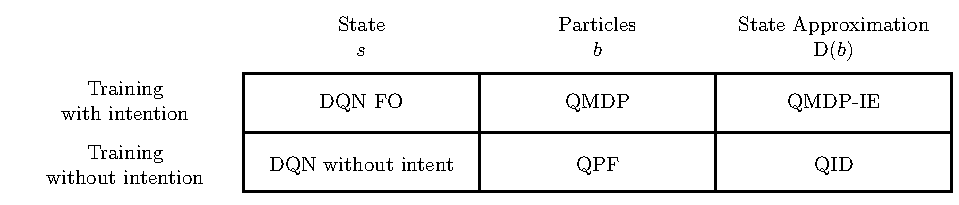
\includegraphics[width=0.85\textwidth]{figures/figures-algorithms.pdf}
%         \begin{tabular}{c}
%         \input{YourThesis/papers/belief/tikz/algo_table}
%         \end{tabular}
        
% \end{table*}

Building upon the belief state $b(s)$ introduced in the previous chapter, our goal is to get an optimal policy $\pi^*$ according to \eqref{eq:optimal_policy} by training a \gls{dqn} using this belief. This section describes our two proposed approaches, QID (intention distribution) and QMDP-IE (intention estimation). 
The proposed approaches are compared with both a naive approach, henceforth referred to as QPF, and an established approximation approach QMDP~\cite{Littman1995}. 
% All four approaches are summarized in Figure~\ref{fig:algorithms}. 
To compare the different approaches fairly, a common \gls{dqn} architecture is used for all four. 
The \gls{dqn} uses a combination of improvement suggestions from~\cite{rainbow}, e.g., double \gls{dqn}~\cite{Hasselt2016ddqn} and experience replay~\cite{Lin1992}, but from here on out is referred to \gls{dqn} for simplicity. The \gls{dqn} used in this work is inspired by the network architecture from our previous work~\cite{tram2019}, shown in Figure~\ref{fig:network}. 
\begin{figure}[!h]
    \centering
        % 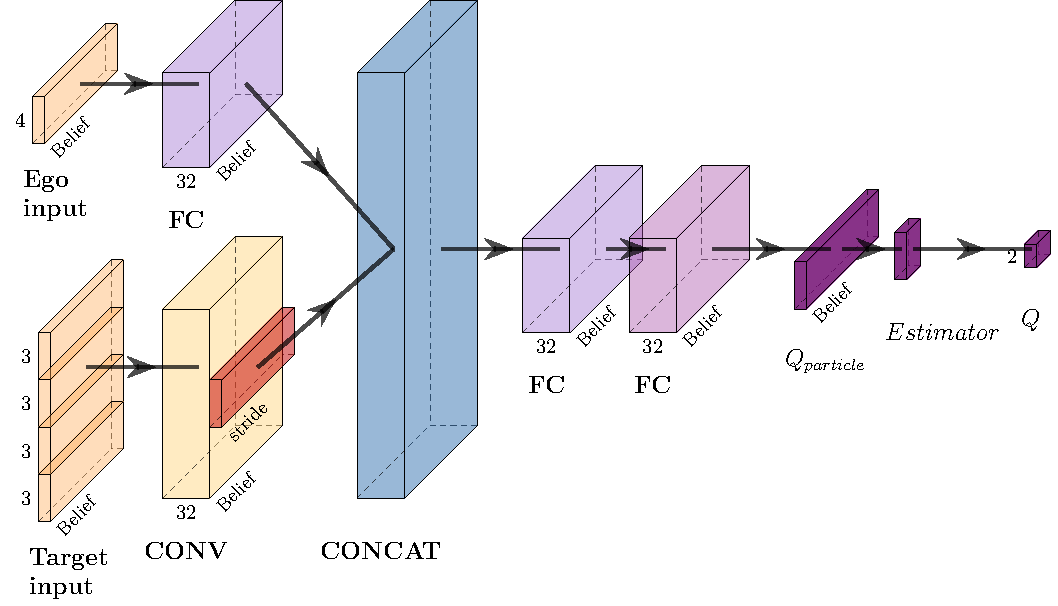
\includegraphics[width=0.9\columnwidth]{figures/belief.pdf}
    \begin{tikzpicture}

    \def\pfx{-1.2};
    \def\pfy{-2.6};
    
    \def\BeliefSize{Z};
    \basenet{6};

    \node[](ego_state) at (-0.8,0.3) {$s_\mathrm{ego}$};
    \node[](target_state) at (-0.8,\pfy+.3) {$s_{1:N}$};
    
    \draw [connection]  ($(input_ego-west)-(1.1,0)$)  -- node {\midarrow} (input_ego-west);
    \draw [connection]  ($(input_target1-southwest)-(1.1,0)$)  -- node {\midarrow} (input_target1-southwest);
    \draw [connection]  (fc2-east)  -- node {\midarrow} ($(fc2-east)+(1.1,0)$);


\end{tikzpicture}
    \caption{Common network architecture, where ego input $s_\mathrm{ego}$ represents the input features for the ego vehicle, and input of all other vehicles $s_{1:N}$. The layers consist of one convolution (Conv), three fully connected (FC), and one concatenation (CONC) layer. Finally, the depth of the layers $Z$ represents the belief size. The network illustrations in this work are generated using \cite{PlotNeuralNet}}.
    \label{fig:network}
\end{figure}

First, the naive approach, QPF, is trained on the entire belief state $b$, as shown in Figure~\ref{fig:qpf}. The observation $o$, is divided into the ego state $s_\mathrm{ego}= (p_\mathrm{ego}^\mathrm{goal},p_\mathrm{ego}^\mathrm{int}, v_\mathrm{ego}, t_\mathrm{stop})$ and the observation of other vehicles $o_{1:N} = \{\hat p_n,\hat v_n \}_{n=1}^N$. The observation of the other vehicles $o_{1:N}$ is sent to the particle filter to update the belief state $b$ and we get the updated particles $x$ according to Algorithm~\ref{alg:particle_filter}. Both $s_\mathrm{ego}$ and $x$ are sent to the \gls{dqn}, where the number of particles $M$ determines the depth $Z$ of the \gls{dqn}, which in turn increases the number of weights as a function of Z. The output of the \gls{dqn} is then sent to a dimension-reducing layer, by calculating the mean value for each action and in turn outputs a single $Q$ vector, denoted as $Q_\mathrm{PF}$. 
As mentioned in the introduction, one challenge with this approach is that the number of particles representing the belief can be very large and this in turn requires more weights which leads to problems for training to converge. 
\begin{figure}[!h]
    \centering
        % \includegraphics[width=0.99\columnwidth]{figures/qpf.pdf}
        \begin{tikzpicture}
    \def\pfx{-1.5}
    \def\pfy{-1.8}
    \def\radius{.95}

    % \node[](obs_text) at (\pfx-1,0) {$o$};
    \node[](obs) at (\pfx-.9,0) {$o$};
    \node[circle, draw=black, minimum size=2.2] (split) at (\pfx, 0) {}; 
    \node[](ego_state) at (.3,0.4) {$\{s_\mathrm{ego} \}_{m=1}^M$};
    \node[](target_state) at (0.2,\pfy+.3) {$\{x_{m} \}_{m=1}^M$};
    \node[](target_observation) at (-1,-.5) {$o_{1:N}$};
    % \node[](target_observation) at (-.5,-.5) {$\{\hat p_n, \hat v_n \}^N_{n=1}$};
    % \node[](target_state) at (-0.5,\pfy+.3) {$\{s_{1:N} \}_{m=1}^M$};
    % \node[](target_state) at (-0.4,-1.3) {$\{x_m\}^M_{m=1}$};
    % \node (intent_state) at (-1, -3) {Intent};
    
    \makepointcloud;
    
    \def\BeliefSize{M};
    \def\BeliefDepth{6};
    
    % \baseinput{6};

    \node[draw,fill=blue!5,thick,inner sep=3pt,minimum width=1mm, minimum height=38mm, dashed, align=center] (dqn) at (1+1,\pfy/2-.3,0){DQN \\ Z=M \\ see \\ Figure \ref{fig:network}};

    
    \pic[shift={(.8,0,0)}] at (dqn.east) 
    {Box={
        name=q_particle,
        caption= ,
        xlabel={{2, }},
        ylabel= ,
        zlabel=\BeliefSize,
        fill=\SoftmaxColor,
        opacity=0.8,
        height=4,
        width=1.5,
        depth=\BeliefDepth
        }
    };

    \pic[shift={(.7,0,0)}] at (q_particle-east) 
    {Box={
        name=q_out,
        caption= ,
        xlabel={{2, }},
        ylabel= ,
        zlabel= 1,
        fill=\SoftmaxColor,
        opacity=0.8,
        height=4,
        width=1.5,
        depth=1
        }
    };
    \draw [connection]  (q_particle-east)  -- node {\midarrow} (q_out-west);
    % \pic[shift={(.4,0,0)}] at (estimator-east) 
    %     {Box={
    %         name=q,
    %         caption=$Q_\mathrm{PF}$,
    %         xlabel={{ , }},
    %         ylabel= ,
    %         zlabel= ,
    %         fill=\SoftmaxColor,
    %         opacity=0.8,
    %         height=2,
    %         width=1.5,
    %         depth=1
    %         }
    %     };
    % \draw [connection]  (estimator-east) -- node {\midarrow} (q-west);
    
    \draw [connection]  (split)  -- node {\midarrow} (pf);
    % \draw [connection]  (obs_text)  -- node {\midarrow} (obs);
    % \draw [connection]  (obs)  -- node {\midarrow} (input_ego-west)
    % \draw [connection]  (pf)  -- node {\midarrow} (input_target1-southwest);
    \draw [connection]  (dqn.east)  -- node {\midarrow} (q_particle-west);
    % \draw [connection]  (input_ego-east)  -- node {\midarrow} ($(input_ego-east)+(1.1,0)$);
    % \draw [connection]  (input_target1-southeast)  -- node {\midarrow} ($(input_target1-southeast)+(1.1,0)$);
    \draw [connection]  (split.east)  -- node {\midarrow} ($(split)+(2.8,0)$);
    \draw [connection]  (obs.east)  -- node {\midarrow} (split.west);
    \draw [connection]  (pf.east)  -- node {\midarrow} ($(pf)+(2.8,0)$);
    \draw [connection]  (q_out-east) -- node {\midarrow} ($(q_out-east)+(.5,0)$);
    \node[](q_pf) at ($(q_out-east)+(1.,0)$) {$Q_\mathrm{PF}$};
    
    \def\dx{.6}
    \def\dy{.4}
    % \def\dy{-1}
    \draw [dashed, thick] (\pfx-\dx,\dy) -- (\pfx-\dx,\pfy-\radius) -- (\pfx+\dx+.3,\pfy-\radius) -- (\pfx+\dx+.3,\dy) -- cycle;
    % \draw [dashed, thick] (\pfx-\dx,\dy) -- (\pfx-\dx,\pfy-\radius) -- (\pfx+\dx,\pfy-\radius) -- (\pfx+\dx,\dy) -- cycle;
    \node[](belief_state) at (\pfx,\pfy-\radius-.3) {\textbf{$b$}};

\end{tikzpicture}\\
        \caption{Block diagram of the QPF algorithm. 
        The belief state $b$ \eqref{eq:particle_belief_state} consists of the observation $o$ and the particles $\{ x_m \}^M_{m=1}$ from the particle filer. From the belief state, the ego state $s_\mathrm{ego}$ is extracted separately from the state of the other vehicles $s_{1:N}=\{ x_m \}^M_{m=1}$ for all cars $1:N$ and feed to the \gls{dqn}, where the depth of the \gls{dqn} is given by the number of particles $M$. After the \gls{dqn} is a depth-reducing layer that reduces the depth M to 1.}
        % Let $b = \{b_m\}_{m=1}^M \in \mathcal{R}^{16\times M}$ be the state for \textbf{all} particles, where ego state $s_\mathrm{ego}$ is extracted separately from the target state $s_{1:N}=\{ x_m \}^M_{m=1}$ for all cars $1:N$, while $M$ is the number of particles and $x_m$ the particle state for particle $m$.}
        % But the weights $\theta= \theta_{\mathrm{PF}}$ are trained using algorithm \ref{alg:training_process} with $b$ in step 5 and  $Q(b, a; \theta_{\mathrm{PF}})$ from \ref{eq:qpf}.
    \label{fig:qpf}
\end{figure}

% This leads us to our first proposed approach, QID, shown in Figure~\ref{fig:qid}. To reduce the input dimensions $Z$ compared to QPF, we propose that the observations $\hat{p}_n$ and $\hat{v}_n$ are fed directly to the \gls{dqn} while the non-observable intention state $\tilde{\zeta}^\mathrm{ID}_n$, is derived from the belief state. For this method, it is simply the marginal distribution of intention from the \discuss{set of particles $\{ x_m \}^M_{m=1}$,} \discuss{thus for QID the state approximation $D(b)$ in Table~\ref{tab:algorithms} is marginalization}: 
This leads us to our first proposed approach, QID, shown in Figure~\ref{fig:qid}. To reduce the input dimensions $Z$ compared to QPF, we propose that the non-observable intention state $\zeta^\mathrm{ID}_n$ is derived from the belief state using an approximator $D(b)$, while the observable states $\hat{p}_n$ and $\hat{v}_n$ are fed directly to the \gls{dqn}. By doing this, the required depth of the \gls{dqn} can be reduced to 1 and is no longer dependent on the number of particles $M$. 
For this method, $\tilde{\zeta}^\mathrm{ID}_n$ is simply the marginal distribution of intention from the set of particles $\{ x_m \}^M_{m=1}$: 
\begin{equation}
    D^\mathrm{ID}(b) = \zeta^\mathrm{ID}_n = \sum_{m=1}^M w_{n[m]} [\zeta_\text{tw} \; \zeta_\text{yd}]_{n[m]},
    \label{eq:ID_i}
\end{equation}
where $w_{n[m]}$ is the weight of the particle $m$ and $[\zeta_\text{tw} , \zeta_\text{yd}]$ is the one-hot vector specifying intention. 

\begin{figure}[!h]
    \centering
        \begin{tikzpicture}
    %\node[](obs_eq) at (-2.5,2) {$o = (p^\mathrm{ego}_\mathrm{goal},p^\mathrm{ego}_\mathrm{int}, v^\mathrm{ego}, t_\mathrm{stop}, \{\hat{p}^{j}_\mathrm{int}, \hat{v}^j\}_{j=1}^N).$};
    %\node (ego_state) at (-0.7, 0.8) {$\hat{s}_e = (p^\mathrm{ego}_\mathrm{goal},p^\mathrm{ego}_\mathrm{int}, v^\mathrm{ego}, t_\mathrm{stop})$};

    % \node (target_state) at (-2.9, -7) {$\hat{s}_j = \{p^{j}_\mathrm{int}, v^j, i^j\}_{j=1}^N$};
    % \node (intent_state) at (-3, -7.5) {Intent from eq.$(20)$};

    %\node (target_state) at (-0.7, -2.5) {$\hat{s}_j = \{p^{j}_\mathrm{int}, v^j\}_{j=1}^N$};
    %\node (intent_state) at (-1, -5.2) {$\hat{i}^j (19)$};

    \def\pfx{-2.2}
    \def\pfy{-1.8}
    \def\radius{.95}

    % \node[](obs) at (\pfx,0) {$o$};
    \node[](ego_state) at (-0.5,0.3) {$s_\mathrm{ego}$};
    % \node[](target_state) at (0.1,-.8) {$\{\hat p_n, \hat v_n \}^N_{n=1}$};
    \node[](target_state) at (-.3,-.8) {$o_{1:N}$};
    \node[](target_observation) at (-1.7,-.8) {$o_{1:N}$};
    \node[](target_state) at (-.5,\pfy+.3) {$\zeta_{n}$};
    \node[](target_state) at (.5,\pfy+.3) {$s_{1:N}$};

        \node[](obs) at (\pfx-.9,0) {$o$};
    \node[circle, draw=black, minimum size=2.2] (split) at (\pfx, 0) {}; 
    % \node[](ego_state) at (.3,0.4) {$\{s_\mathrm{ego} \}_{m=1}^M$};
    % \node[](target_state) at (0.2,\pfy+.3) {$\{x_{m} \}_{m=1}^M$};
    % \node[](target_observation) at (-1,-.5) {$o_{1:N}$};
    
    \makepointcloud

    \def\BeliefSize{1}
    \def\BeliefDepth{1}
    % \baseinput{1};

    \node[draw,fill=blue!5,thick,inner sep=3pt,minimum width=1mm, minimum height=38mm, dashed, align=center] (dqn) at (2,\pfy/2-.3,0){DQN \\ Z=1 \\ See \\ Figure \ref{fig:network}};

    
    \pic[shift={(0.5,0,0)}] at (dqn.east) 
    {Box={
        name=q_particle,
        caption=,
        xlabel={{2, }},
        ylabel= ,
        zlabel=\BeliefSize,
        fill=\SoftmaxColor,
        opacity=0.8,
        height=4,
        width=1.5,
        depth=\BeliefDepth
        }
    };

    \pic[shift={(1.1,0,0)}] at (pf) 
    {Box={
        name=approx,
        caption=$ $,
        xlabel={{ , }},
        ylabel= ,
        zlabel= ,
        fill=\SoftmaxColor,
        opacity=0.8,
        height=4,
        width=1,
        depth=\BeliefDepth
        }
    };

    \draw [connection]  (dqn.east)  -- node {\midarrow} (q_particle-west);
    % \draw [connection]  (input_ego-east)  -- node {\midarrow} ($(input_ego-east)+(1.1,0)$);
    % \draw [connection]  (input_target1-southeast)  -- node {\midarrow} ($(input_target1-southeast)+(1.1,0)$);
    %\node (space) at (,0) {};		
    \draw [connection]  (split)  -- node {\midarrow} (pf);
    \draw [connection]  (obs)  -- node {\midarrow} (split);
    % \draw [connection]  (obs)  -- node {\midarrow} (input_ego-west);
    % \draw [connection]  (obs)  -- node {\midarrow} (input_target1-southwest);
    \draw [connection]  (split)  -- node {\midarrow} ($(split)+(3.35,0)$);
    \draw [connection]  (split)  -- node {\midarrow} ($(approx-east)+(1.2,0)$);
    \draw [connection]  (pf)  -- node {\midarrow} (approx-west);
    \draw [connection]  (approx-east)  -- node {\midarrow} ($(approx-east)+(1.2,0)$);
    \draw [connection]  ($(approx-east)+(1.2,0)$)  -- node {\midarrow} ($(approx-east)+(2.35,0)$);
    \draw [connection]  (q_particle-east) -- node {\midarrow} ($(q_particle-east)+(.5,0)$);
    \node[](q_pf) at ($(q_particle-east)+(.8,0)$) {$Q$};
    
    % \def\dx{.55}
    % \def\dy{.2}
    % % \draw [dashed, thick] (\pfx-\dx,\dy) -- (\pfx-\dx,\pfy-\radius) -- (\pfx+\dx+.6,\pfy-\radius) -- (\pfx+\dx+.6,\dy) -- cycle;
    % \draw [dashed, thick] (\pfx-\dx,\dy) -- (\pfx-\dx,\pfy-\radius) -- (\pfx+\dx,\pfy-\radius) -- (\pfx+\dx,\dy) -- cycle;
    % \node[](belief_state) at (\pfx,\pfy-\radius-.3) {\textbf{$b$}};
    % \node[](belief_state) at (\pfx+.3,\pfy-\radius-.3) {\textbf{$D(b)$}};
    \def\dx{.6}
    \def\dy{.4}
    % \def\dy{-1}
    \draw [dashed, thick] (\pfx-\dx,\dy) -- (\pfx-\dx,\pfy-\radius) -- (\pfx+\dx+.3,\pfy-\radius) -- (\pfx+\dx+.3,\dy) -- cycle;
    % \draw [dashed, thick] (\pfx-\dx,\dy) -- (\pfx-\dx,\pfy-\radius) -- (\pfx+\dx,\pfy-\radius) -- (\pfx+\dx,\dy) -- cycle;
    \node[](belief_state) at (\pfx,\pfy-\radius-.3) {\textbf{$b$}};
    \node[](belief_state) at (\pfx+1.3,\pfy-\radius+0.2) {\textbf{$D(b)$}};
\end{tikzpicture}
        % \vspace{-1cm}
        \caption{Our proposed approaches, QID and QMDP-IE. From an observation $o$, the observable states $s_\mathrm{ego}$ and $o_{1:N}=\{\hat{p}_n, \hat{v}_n\}_{n=1}^N$ are fed directly to the network. While an approximator $D(b)$ approximates the non-observable intention state $\hat \zeta_n$, so that $s_{1:N}=\{\hat p_n, \hat v_n, \hat \zeta_n \}^N_{n=1}$.
        % and combined with the observable states $\{\hat p_n, \hat v_n \}^N_{n=1}$ we get $s_n=\{\hat p_n, \hat v_n, \hat \zeta_n \}^N_{n=1}$.
        }
    \label{fig:qid}
\end{figure}

Another way to reduce the depth of the \gls{dqn} and still consider the uncertainty of non-observable states is the approximation method QMDP~\cite{Littman1995}. Where the weights $\theta_\mathrm{MDP}$ are trained in an environment with full observability. This can be used when the non-observable states can be identified offline e.g., using ground truth labeling. During evaluation time, each particle represents one belief state $b_m = \{ s_{ego}, \{x_{n[m]}\}_{n=1}^N  \}$ and is evaluated using $\theta_\mathrm{MDP}$ and the approximated Q-value of the entire belief state is given by \ref{eq:qmdp} 
\begin{equation}
    Q(b, a) \approx \frac{1}{M} \sum_m Q_{\mathrm{MDP}}(b_{m}, a; \theta_\mathrm{MDP}).
\end{equation}
% However, the resulting policy can be sensitive to the performance of the state estimation algorithm used to generate the belief state $b$. 

While QMDP reduces the required depth of the network, all $M$ particles are still processed through the network and require $M$ number of operations more than QID. 
This leads us to our final proposed approach, QMDP-IE. If we had access to $\theta_\mathrm{MDP}$, instead of averaging the Q-values of all the particles, a threshold $\zeta_\text{threshold}$ is set on the intention distribution from the particle filter and then use it as the true intention state. 
Similar to QID, the particle filter is only used to generate the intention and is represented as a one-hot vector
\begin{align}
D^\mathrm{IE}(b) = \hat{\zeta}^\mathrm{IE}_n = & \begin{cases}
[0 \; 1] & \text{if} \ \tilde{\zeta}_n^\text{yd} > \zeta_\text{threshold},\\
[1 \; 0] & \text{otherwise,}
\label{eq:IE_i}
\end{cases} 
\end{align}
where $\zeta_\text{threshold}$ is a design parameter that can be adjusted offline without any retraining of the \gls{dqn} and directly correlates with the aggressiveness of the policy, e.g., a high value on $\zeta_\text{threshold}$ makes the agent more passive. 

% All four approaches are shown in Table~\ref{tab:algorithms} and the next chapter describes the experiment setup used to compare the different approaches. 
\begin{table}[!h]
\begin{tabular}{ccc}
\multicolumn{1}{l}{} & \begin{tabular}[c]{@{}c@{}}Particles \\ $b$\end{tabular} & \begin{tabular}[c]{@{}c@{}}State Approximation \\ $\text{D}(b)$ \end{tabular} \\ \cline{2-3} 
\multicolumn{1}{c|}{\begin{tabular}[c]{@{}c@{}}\\[1pt] Training\\ weights $\theta$ \\[5pt] \end{tabular}}          & \multicolumn{1}{c|}{\textit{QPF}, $\theta_\mathrm{PF}$}           & \multicolumn{1}{c|}{\textbf{QID}, $\theta_\mathrm{ID}$}        \\ \cline{2-3} 
\multicolumn{1}{c|}{\begin{tabular}[c]{@{}c@{}}\\[1pt] Weights $\theta_\mathrm{MDP}$ \\ from ground truth \\[5pt] \end{tabular}} & \multicolumn{1}{c|}{\textit{QMDP}, $\theta_\mathrm{MDP}$}         & \multicolumn{1}{c|}{\textbf{QMDP-IE}, $\theta_\mathrm{MDP}$}   \\ \cline{2-3} 
\end{tabular}
\caption{The difference between the \textbf{investigated algorithms}, while the other two are used as benchmarks. The columns show the algorithm's input to the neural network, where the first column contains the \textit{baseline algorithms} that use the belief state $b$ with all $M$ particles and the second column contains algorithms that use an estimate of the intention. The first row shows the algorithms that train the weights with the given input and the second row shows algorithms that use weights trained on full observability.}
\label{tab:algorithms}
\end{table}

\begin{algorithm}[!t]
    \caption{double Q-learning training process}\label{alg:training_process}
    \begin{algorithmic}[1]
        \State Initialize $\theta$ randomly
        \State $\mathcal{D} \gets \emptyset$
        % \State $t \gets 0$
        \For{nr episodes}
            \State $o \gets $ initiate environment
            \Comment{\eqref{eq:observation}}
            \State $b \gets $ \Call{InitializeBelief}{$o$}
            \Comment{Alg. \ref{alg:init_particle_filter}}
            \While{episode not finished}
                \If{$e \sim \mathcal{U}(0,1) < \epsilon$}
                    \Comment{from~\cite{Mnih2013}}
                    \State $a \gets \mathrm{random\ action}$
                \Else
                    \State $Q(b, a) \gets $\Call{GetActionValues}{$b, \theta$}
                    \Comment{S.~\ref{sec:belief_rl_algo}}
                    \State $a \gets \argmax_{a} Q(b,a)$
                    \Comment{\eqref{eq:optimal_policy}}
                \EndIf
                \State $o^\prime, r \gets $ \Call{StepEnvironment}{$a$}
                \Comment{S.~\ref{sec:simulation_setup}}
                \State $b^\prime \gets $ \Call{UpdateBelief}{$b$, $o^\prime$, $a$}
                \Comment{Alg. \ref{alg:particle_filter}}
                \State $\mathcal{D} \gets \mathcal{D} \cup \{(b, a, r, b^\prime)\}$
                % \Comment{from~\cite{Lin1992}}
                \State $E \gets $ sample from $\mathcal{D}$
                \Comment{from~\cite{Lin1992}}
                \State update $\theta^-$ with SGD and loss $J(\theta,\theta^-)$ 
                \Comment{\eqref{eq:ddqn-loss}}
                \For{every $N_\mathrm{update}$}
                    \State update $\theta$ with $\theta^-$
                    \Comment{from~\cite{Hasselt2016ddqn}}
                \EndFor
            % \State $t \gets t + 1$
            \EndWhile
        \EndFor
        % \Function{UpdateBelief}{$b_t, \theta$}
        % 
        % \EndFunction
    \end{algorithmic}
\end{algorithm}

All four approaches are shown in Table~\ref{tab:algorithms} and the weights $\theta_\mathrm{PF}$, $\theta_\mathrm{ID}$ and $\theta_\mathrm{MDP}$ are obtained using double deep Q-learning~\cite{Hasselt2016ddqn}, described in Algorithm~\ref{alg:training_process}, where step $10$ is different between the algorithms. Step 12 is the simulator described in the next section while step 13 is the particle filter update described in Algorithm~\ref{alg:particle_filter}. $\mathcal{D}$ in step $14-15$, is an experience replay buffer that makes the convergence of \gls{dqn} more robust~\cite{Mnih2015}.
The loss function in step $16$ modifies \eqref{eq:dqn-loss} to
\begin{equation}
    J(\theta,\theta^-) = \mathbb{E}[(r + \gamma Q(s,\argmax_{a} Q(s,a;\theta);\theta^-)],
    % J(\theta,\theta^-) = E_{s^\prime}[(r + \gamma Q(s',\argmax_{a'} Q(s',a';\theta);\theta^-)],
    \label{eq:ddqn-loss}
\end{equation}
where $\theta^-$ is the weight of the target network. 

All algorithms are trained and evaluated on the same simulator and are described in the next section. 

% \begin{figure*}[!t]
%     \centering
%         \hspace*{-4cm}%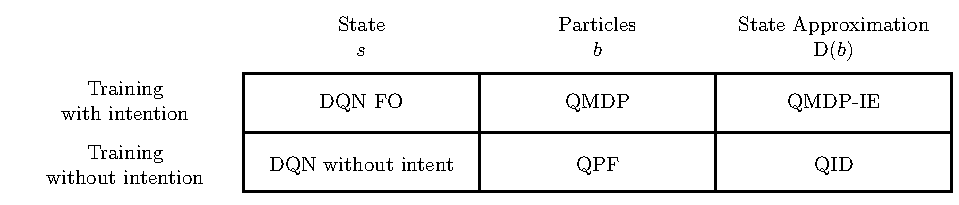
\includegraphics[width=0.85\textwidth]{figures/figures-algorithms.pdf}
%         \input{YourThesis/papers/belief/tikz/algo_table}
%         \caption{Table showing the difference between proposed algorithms. The first row are algorithms that have access to the true intention during training, while the algorithms on the second row do not. The columns show the input to the neural network, where the first column contains the baseline algorithms that use the noisy observation from the sensors either with or without the intention $\zeta_n$. The second column contains algorithms using all $M$ particles as input and the final column uses an estimate of the intention.}
%     \label{fig:algorithms}
% \end{figure*}

\section{Experiments}
\label{sec:experiments}
The main goal of the experiments is to show the performance difference between the algorithms described in the previous chapter. 
In this section, we present the experiment setup in three parts. First, we describe how the simulator generates the different traffic scenarios. Second, the design of the reward function with some motivation to its values is described. Finally, we define the common network architecture, shown in Figure~\ref{fig:network}.
%This section describes the experiment setup. We start by describing how the simulator generates the different traffic scenarios, then we define the network architecture and the training procedure.

\subsection{Simulator setup}
\label{sec:simulation_setup}

Starting with the simulator, at the start of each episode, up to $N$ vehicles are spawned with some initial values. The number of vehicles simultaneously in the other lane is the same thing as the traffic density of the lane. The initial positions $p_n^0$ are distributed along the intersecting lane with the furthest distance from the intersection being $p_\mathrm{lim}$, a starting velocity $v_n^0$, and a desired velocity $v^\mathrm{desired}_n$. Each vehicle is spawned with a deterministic policy that represents its intention $\zeta_n$, which can either be $\zeta_n^\mathrm{tw}$ \textit{take way} or $\zeta_n^\mathrm{yd}$ \textit{yield}. These intentions follow the same transition model as the actions described in Section~\ref{sec:action} for the ego vehicle and the time between simulation steps is $\mathrm{d}t_{\text{decision}}$ seconds.
The ego vehicle is spawned last with an initial speed $v_\mathrm{ego}$ and desired speed $v_\mathrm{ego}^\mathrm{desired}$, i.e., $v^\mathrm{desired}_n$ from \eqref{eq:idm}. 

% The simulator keeps track of the true state $s$ of all objects and an observation model is used to add noise to each observation, according to \eqref{eq:noise_pos} and \eqref{eq:noise_vel}. 
Every time a vehicle in the perpendicular lane crosses the intersection, they are removed and a new vehicle is spawned at the start of the lane at a random time with new initial values $p_n^0, v_n^0, v^\mathrm{desired}_n$ and intention $\zeta_n$. 

As mentioned in the introduction, the scenario from our previous work \cite{tram2019} that had the most difficulty solving was a \textit{conflict scenario}, i.e., when another vehicle in the crossing lane has the same velocity and the same distance to the intersection. To create these conflict scenarios, the starting position of ego $p^0_\mathrm{ego}$ is set based on the time to intersection $\tau_{tti}$ of one of the other vehicles.
This "other car" is referred to as the conflict car and is randomly chosen. 
% This "other car" is referred to as the conflict car, as shown in Figure~\ref{fig:conflict_car}, and is randomly chosen. 
% The initial position of the ego becomes: 
% \begin{equation}
%     p_\mathrm{ego}^{0} = v_\mathrm{ego} \frac{p^{c}_{0}}{v^{c}_{0}},
% \end{equation}
% where $c$ is the index of the conflict car.
This increases the probability that the ego will be in conflict with at least one other car. 

Each episode is simulated until a terminal state, 
\begin{enumerate*}[label=(\roman*)]
  \item goal,
  \item collision, 
  \item safe stop, 
  \item or deadlock, 
\end{enumerate*} and a reward is given according to the reward function.

\begin{table}[!h]
    % increase table row spacing, adjust to taste
    % \renewcommand{\arraystretch}{1.2}
    \caption{Hyperparameters of Simulator}
    \label{tab:hyperparameters}
    \centering
    \begin{tabular}{l l r}
        \toprule
        %Parameter & Value\\
        % sampling time [\unit{\second}], & $\mathrm{d}t_\mathrm{sampling}$ & $0.5$\\
        decision time [\unit{\second}], & $\mathrm{d}t$ & $2$\\
        maximum initial distance [\unit{\meter}], & $p_\mathrm{lim}$ & $50$\\ 
        initial speed [\unit{\meter\per\second}], & $v^0_n $ & $2-7$\\
        initial acceleration [\unit{\meter\per\second\squared}], & $a^0_n $ & $0$\\
        desired speed [\unit{\meter\per\second}], & $v^\mathrm{desired}_n$ & $2-7$\\
        time gap [\unit{\second}], & $T_\mathrm{gap}$ & $1.5$\\
        Stop time limit [\unit{\second}], & $T_\mathrm{stop}$ & $10$\\
        % Timeout time [\unit{\second}], & $T_\mathrm{lim}$ & $120$\\
        ego initial speed [\unit{\meter\per\second}], & $v_\mathrm{ego}$ & $5$\\
        ego desired speed [\unit{\meter\per\second}], & $v_\mathrm{ego}^\mathrm{desired}$ & $5$\\
        noise position [\unit{\meter}], & $\sigma_\mathrm{p}$ & $2$\\ 
        noise velocity [\unit{\meter\per\second}], & $\sigma_\mathrm{v}$ & $1$\\ 
        max observed vehicles, & $N$ & $4$\\ 
    
            \midrule
            IDM max acceleration [\unit{\meter\per\second\squared}], & $\alpha^{\mathrm{max}} $ & $0.73$\\
            IDM deceleration [\unit{\meter\per\second\squared}], & $\alpha_b $ & $0.5 - 4.0$\\
            IDM acceleration exponent, & $\delta$ & $4$\\
            IDM minimum distance [\unit{\meter}], & $d_0$ & $2$\\
            IDM vehicle length [\unit{\meter}], & $l_n$ & $4$\\
        \midrule
        
        number of particles & $M$ & 100\\
        min number of particles & $M_\mathrm{threshold}$ & 75\\
        acceleration noise [\unit{\meter\per\second\squared}] & $\sigma_a$ & 0.1 \\
        intention switch probability [$\%$] & $\xi_i$ & 5 \\
        intention probability threshold & $\zeta_\text{threshold}$ & 0.8 \\
        \midrule
        
        Batch size & B & $128$ \\
        Learning rate & lr & $0.0001$ \\
        Discount factor & $\gamma$ & $0.95$\\
        Replay memory size & $E_\mathrm{replay}$ & $20{,}000$\\
        Target network update frequency & $N_\mathrm{update}$ & $1{,}000$\\
    
    % 		Initial exploration constant, $\epsilon_\mathrm{start}$  & $1$\\
    % 		Final exploration constant, $\epsilon_\mathrm{end}$ & $0.05$\\
    % 		Final exploration iteration, $N_{\epsilon\mathrm{{\mathrm -}end}}$ & $1{,}000{,}000$\\
    
            \bottomrule
        \end{tabular}
    \end{table}

\subsection{Designing the reward function}
The reward function $R$ is part of the \gls{pomdp} defined in Section~\ref{sec:pomdp_formulation} and the reward for each terminal state determines the behavior of the optimal policy $\pi^*$ from \eqref{eq:optimal_policy}. 
According to \cite{Hasselt2016}, large reward values would result in large Q-values, which can cause the gradients to grow. With some trial and error, the rewards for each terminal state for this \gls{pomdp} are defined as
\begin{align*}
r = & \begin{cases}
\hfill 8 & \text{reaching the goal},\\
\hfill -10 & \text{collision},\\
\hfill 0.4 & \text{safe stop},\\
\hfill -0.6 & \text{deadlock}, \\
-0.01 & \text{non-terminal states}.
\label{eq:reward_values}
\end{cases} 
\end{align*}
% The possible terminal states are the following:
% \begin{enumerate*}[label=(\roman*)]
%   \item Goal, ego vehicle reaching the goal;
%   \item Collision, ego collides with one of the other vehicles;
%   \item Safe stop, if the ego vehicle has been standing still for more than $T_\mathrm{stop}$ seconds and no other car is standing still;
%   \item Deadlock, if another vehicle standing still at the intersection yielding for the ego vehicle and while the ego vehicle has also been standing still for more than $T_\mathrm{stop}$ seconds; 
%   % \item Timeout, if the total simulation time exceeds $T_{lim}$. 
% \end{enumerate*}
% As defined by the reward function in \eqref{eq:reward_function}, each terminal state has a corresponding reward
% \begin{align*}
% r = & \begin{cases}
% \hfill 8 & \text{reaching the goal,}\\
% \hfill -10 & \text{collision},\\
% \hfill 0.4 & \text{safe stop,}\\
% \hfill -0.6 & \text{deadlock}, \\
% -0.01 & \text{non-terminal states}.
% \label{eq:reward_values}
% \end{cases} 
% \end{align*}
To get a policy that can cross the intersection when possible, a high reward of $r=8$ is received whenever the agent reaches the goal. A high negative reward of $r=-10$ is received when the agent collides with another car to ensure that it avoids collisions. 
% While goal and collision states can only be reached if the policy chooses to cross the intersection by taking the take way action enough times, 

When the agent instead chooses to yield and stop for longer than $T_\mathrm{stop}$ seconds, the received reward depends on what the other vehicle did. 
While the agent has stopped and the cars on the intersecting lane are crossing the intersection, the agent has made a safe stop and receives the reward $r=0.4$. To disincentivize deadlock situations, where two cars are waiting for each other, a small negative reward is received $r=-0.6$. 

Finally, to incentivize the agent to quickly reach a terminal state, a small negative reward is given for each decision step when the agent has not reached a terminal state combined with the discount factor $\gamma$. 

% The motivation for the goal reward being $8$ in contrast to $-10$ is to make the policy a little more passive and choose yield when the probability distribution is close to $50\%$. For example, in a simplified case when the terminal state is only dependent on the intention and the distribution of the intention in the belief state is evenly distributed, the Q-value would be $Q(b, a) \approx [-1 \; -.1]$, i.e., the expected reward for taking action \textit{take way} is $-1$ and $-.1$ for taking the action \textit{yield} according to \eqref{eq:qmdp}. 
% % \begin{equation}
% %     \frac{50*8 + 50*-10}{100} = -1
% %     \frac{50*.4 + 50*-.6}{100} = -.1
% %     8x + (100-x)*-10 > .4x + (100-x)*-.6
% %     x > 44.4444
% % \end{equation}
% Following the same simple example, it would require about $55\%$ of the belief state to be yield for the Q-value to be higher for \textit{take way} than \textit{yielding}.

% The terminal state referred to as collision in this paper may sound drastic, but what is represented as a collision in simulation can be interpreted as an intervention by a collision avoidance system when implemented in real world.



\section{Results and discussion}\label{sec:results}
This section presents the evaluation metrics and results from the experiments, described in Section~\ref{sec:simulation_setup}. 
% Because the scenario with four other cars is the hardest to cross without colliding, it is used to compare the performance of the different agents.
Each algorithm is evaluated on \num{2000} episodes. 
The initial values, defined in Table~\ref{tab:hyperparameters}, were randomized using the episode number as a seed. The defined seed number ensures the same scenarios are used when comparing the different algorithms. 
% The random seeds are based on the episode number, which generates the same values for the random parameters, defined in Table~\ref{tab:hyperparameters}, for each test scenario when evaluating different agents.
The metrics of interest are the average time it takes for the agent to reach the success state and how often each terminal state is reached. A success state refers to either reaching the goal or a safe stop. An ideal agent would cause no collisions or deadlocks, and pass the junction with the smallest possible success time.

Another way to describe the algorithms' performance is by using aggressive and passive, which are not completely complementary to each other. An agent is considered aggressive if it has a low success time but a higher collision percentage, when compared to the Oracle DQN. An agent that does not collide often but instead ends up in deadlock more often is considered passive. So an agent that has low success time and high no collisions is neither aggressive nor passive, just a good agent.
We start with analyzing how well a \gls{dqn} agent that does not consider intentions, performs in scenarios with different traffic densities. 
% Starting with analyzing the traffic density in scenarios and showing its difficulty when not considering intentions. 



\subsection{Traffic density experiment}
\begin{figure}[!h]
    \centering
        % \includegraphics[width=0.99\columnwidth]{figures/results Scenarios 1-5 Take way Cars wo intent.png}
        % This file was created with tikzplotlib v0.10.1.
\begin{tikzpicture}

\definecolor{darkgray176}{RGB}{176,176,176}
\definecolor{goldenrod1911910}{RGB}{191,191,0}
\definecolor{green01270}{RGB}{0,127,0}
\definecolor{lightgray204}{RGB}{204,204,204}

\begin{groupplot}[group style={group size=1 by 2}]
\nextgroupplot[
height=3.5cm,
scaled x ticks=manual:{}{\pgfmathparse{#1}},
tick align=outside,
tick pos=left,
width=7cm,
x grid style={darkgray176},
xmin=-0.2, xmax=4.2,
xtick style={color=black},
ytick={13,15,17,19,21},
xtick={0,1,2,3,4},
xticklabels={1 car,2 cars,3 cars,4 cars,5 cars},
xticklabels={},
y grid style={darkgray176},
ylabel={Success Time [s]},
ymin=13, ymax=21,
ytick style={color=black}
]
\addplot [semithick, black, mark=*, mark size=3, mark options={solid}]
table {%
0 13.5619959677419
1 16.9007190265487
2 20.5162469536962
3 20.4080622347949
4 19.7671118530885
};

\nextgroupplot[
height=3.5cm,
legend cell align={left},
legend style={
  fill opacity=0.8,
  draw opacity=1,
  text opacity=1,
  at={(1,0.5)},
  anchor=west,
  draw=lightgray204
},
tick align=outside,
tick pos=left,
width=7cm,
x grid style={darkgray176},
xmin=-0.2, xmax=4.2,
xtick style={color=black},
xtick={0,1,2,3,4},
xtick={0,1,2,3,4},
xtick={0,1,2,3,4},
xtick={0,1,2,3,4},
xtick={0,1,2,3,4},
xticklabels={1 car,2 cars,3 cars,4 cars,5 cars},
xticklabels={1 car,2 cars,3 cars,4 cars,5 cars},
xticklabels={1 car,2 cars,3 cars,4 cars,5 cars},
xticklabels={1 car,2 cars,3 cars,4 cars,5 cars},
xticklabels={1 car,2 cars,3 cars,4 cars,5 cars},
y grid style={darkgray176},
ylabel={Outcome [\%]},
ymin=-1, ymax=100,
ytick style={color=black}
]
\addplot [semithick, green01270, mark=*, mark size=3, mark options={solid}]
table {%
0 99.2
1 90.4
2 61.55
3 35.35
4 29.95
};
\addlegendentry{goal}
\addplot [semithick, goldenrod1911910, mark=square*, mark size=3, mark options={solid}]
table {%
0 0
1 0.75
2 21.6
3 49.5
4 53.25
};
\addlegendentry{safestop}
\addplot [semithick, red, mark=diamond*, mark size=3, mark options={solid}]
table {%
0 0.8
1 8.85
2 16.85
3 15.15
4 16.8
};
\addlegendentry{collision}
\addplot [semithick, blue, mark=triangle*, mark size=3, mark options={solid}]
table {%
0 0
1 0
2 0
3 0
4 0
};
\addlegendentry{deadlock}
\end{groupplot}

% \draw ({$(current bounding box.south west)!0.5!(current bounding box.south east)$}|-{$(current bounding box.south west)!0.98!(current bounding box.north west)$}) node[
%   scale=0.5,
%   anchor=north,
%   text=black,
%   rotate=0.0
% ]{Scenarios 1-5 Take way Cars wo intent};
\end{tikzpicture}

        \vspace{-0.8cm}
        \caption{Performance results for DQN without intention state $\zeta$, showing success time and outcome percentage for scenarios with increasing numbers of other cars.}
    \label{fig:number_cars}
\end{figure}
Traffic density affects the problem at hand. Figure~\ref{fig:number_cars} shows the results from an experiment with \gls{dqn} trained agents that do not consider intentions in scenarios with different traffic densities. The 1-car scenario corresponds to traffic densities up to 1 car or vehicle per 50 m, or 20 vehicles/km; 2 cars correspond to 2 cars per 50 m, 40 vehicles/km, and so on. The results presented in Figure~\ref{fig:number_cars} clearly show that for low traffic densities, the problem can relatively easily be solved without needing intention estimation. The agent can solve the problem without collisions, deadlocks, or safe stops. As the traffic density increases, the performance significantly drops. For traffic densities larger than 60 vehicles/km (4 cars), the agent only reaches the goal in approximately \SI{35}{\percent} of the cases, makes safe stops before the intersection in \SI{50}{\percent} of the cases, and collides in \SI{15}{\percent}, which makes them the scenarios that can be most improved upon with algorithms that consider intentions. This experiment also gives a sense of the limit of how a \gls{dqn} can perform when not considering the intention state $\zeta$.

As traffic densities in OECD countries according to \cite{OECD} is around 60 vehicles/km, the rest of the experiments will focus on the 4 cars scenario. 


\begin{table}[!h]
\caption{Result summary for 4 cars scenario}
\label{tab:results_summary}
\begin{tabularx}{\columnwidth}{@{}l*{10}{c}c@{}}
\toprule
Experiments     & Goal    & Safe & Collision & Deadlock & Success & Training \\ 
                & reached & stop &           &          &  time   & time\\ 
     & $\%$ & $\%$ & $\%$ & $\%$ & s & h\\ 
\midrule
Oracle DQN    & $84.50$ & $14.45$ & $1.05$ & $0.00$ & $15.49$ & $31\unit{\hour}$ \\ % $1\unit{\day}7\unit{\hour}$ \\ 
% Noisy DQN & $84.25$ & $14.10$ & $1.65$ & $0.00$ & $15.48$ \\ 
\textbf{QMDP-IE}   & $\textbf{80.00}$ & $\textbf{18.15}$ & $\textbf{1.35}$ & $\textbf{0.50}$ & $\textbf{17.14}$ & \textbf{N/A} \\ 
% QMDP-IE   & $80.30$ & $16.20$ & $3.30$ & $0.20$ & $16.54$ & N/A \\ 
QMDP      & $71.95$ & $15.05$ & $5.70$ & $7.30$ & $20.56$ & N/A\\ 
% \arrayrulecolor{red}\hline
% \arrayrulecolor{black}
\textbf{QID}       & $\textbf{85.60}$ & $\textbf{10.40}$ & $\textbf{3.70}$ & $\textbf{0.30}$ & $\textbf{16.64}$ & $\textbf{119\unit{\hour}}$ \\ %$\textbf{5\unit{\day}5\unit{\hour}}$ \\ 
QPF       & $63.50$ & $21.80$ & $12.15$ & $2.55$ & $16.61$ & $124\unit{\hour}$ \\ % $5\unit{\day}4\unit{\hour}$\\ 

\bottomrule
\end{tabularx}
\end{table}


\subsection{Probability distribution of the intention state}
\begin{figure*}[!t]
    \begin{subfigure}[b]{0.24\textwidth}
         \centering
         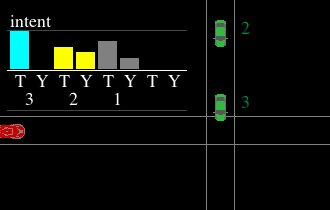
\includegraphics[width=0.99\textwidth]{figures/intent_distribution/screenshot_2.jpeg}
         \caption{$t=0$}
         % \label{fig:y equals x}
     \end{subfigure}
     \hfill
     \begin{subfigure}[b]{0.24\textwidth}
         \centering
         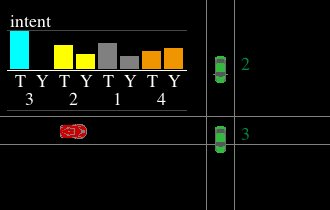
\includegraphics[width=0.99\textwidth]{figures/intent_distribution/screenshot_3.jpeg}
         \caption{$t=1$}
         % \label{fig:three sin x}
     \end{subfigure}
     \hfill
     \begin{subfigure}[b]{0.24\textwidth}
         \centering
         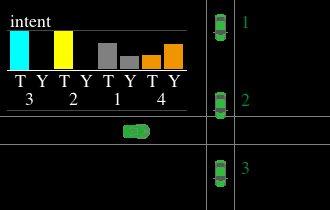
\includegraphics[width=0.99\textwidth]{figures/intent_distribution/screenshot_4.jpeg}
         \caption{$t=2$}
         % \label{fig:screenshot3}
     \end{subfigure}
     \begin{subfigure}[b]{0.24\textwidth}
         \centering
         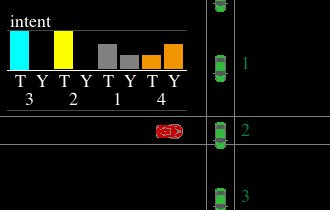
\includegraphics[width=0.99\textwidth]{figures/intent_distribution/screenshot_5.jpeg}
         \caption{$t=3$}
         % \label{fig:screenshot4}
     \end{subfigure}
     \hfill
     \begin{subfigure}[b]{0.24\textwidth}
         \centering
         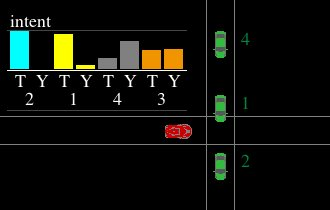
\includegraphics[width=0.99\textwidth]{figures/intent_distribution/screenshot_6.jpeg}
         \caption{$t=4$}
         % \label{fig:y equals x}
     \end{subfigure}
     \hfill
     \begin{subfigure}[b]{0.24\textwidth}
         \centering
         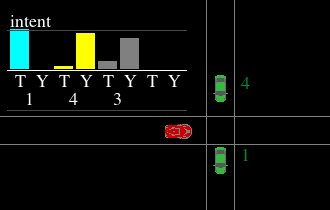
\includegraphics[width=0.99\textwidth]{figures/intent_distribution/screenshot_7.jpeg}
         \caption{$t=5$}
         % \label{fig:three sin x}
     \end{subfigure}
     \hfill
     \begin{subfigure}[b]{0.24\textwidth}
         \centering
         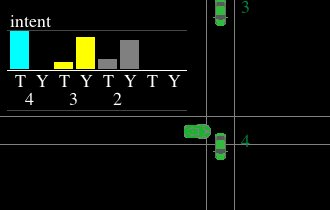
\includegraphics[width=0.99\textwidth]{figures/intent_distribution/screenshot_8.jpeg}
         \caption{$t=6$}
         % \label{fig:screenshot3}
     \end{subfigure}
     \begin{subfigure}[b]{0.24\textwidth}
         \centering
         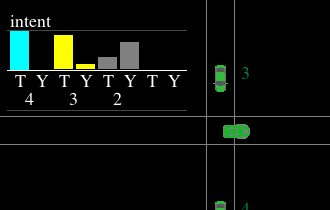
\includegraphics[width=0.99\textwidth]{figures/intent_distribution/screenshot_9.jpeg}
         \caption{$t=7$}
         % \label{fig:screenshot4}
     \end{subfigure}
     
    \centering
        % \hspace*{-4cm}%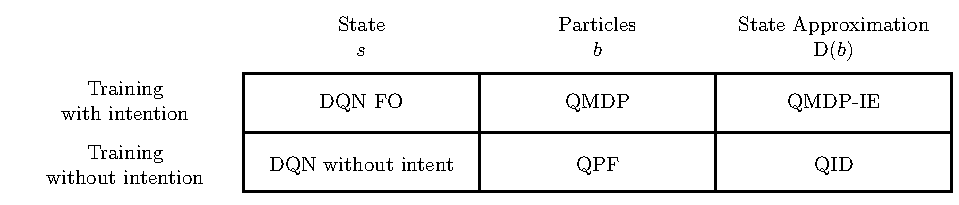
\includegraphics[width=0.85\textwidth]{figures/figures-algorithms.pdf}
        % \input{YourThesis/papers/belief/tikz/algo_table}
        \caption{Example with a QMDP agent. 
        % The car on the left driving horizontally is ego. When ego car is green it is taking the take way action and red when it is taking the yield action. 
        The numbers on the right of the vertical cars are the cars id number $n$. The intention bar figure in each image shows the intention distribution for each other car. Each car has two bars grouped by the same color and the car id number, starting with the take way probability on the left and marked by a "T" and yield probability on the right marked with a "Y".}
        % \vspace{-1cm}
    \label{fig:qmdp_screenshot}
\end{figure*}
The particle filter generates the probability distribution of the non-observable intention state $\zeta$, which can be used to make the algorithms from Section~\ref{sec:belief_rl_algo} possible to implement. 

In Figure~\ref{fig:qmdp_screenshot}, an example of a QMDP agent with the intention distribution from the particle filter is shown. Looking at the first car with id 3 at $t=0-3$, we can observe that the particle filter correctly predicts the take way intention and has some uncertainty about the intention for car id 2 and 1 crossed the intersection. 
% This confirms that the particle filter behaves in a desirable way. 
It is also interesting to observe car id 4, as it temporarily has a higher probability of yielding when following car id 1 for $t=1-5$, but could quickly switch to take way once car 1 crossed the intersection at $t=6$. 

The example from Figure~\ref{fig:qmdp_screenshot} shows that the proposed particle filter performs well at estimating the probability distribution of the intention. However, it relies on an accurate prediction model and could make some mistakes. 
Because we want to investigate if the approximation of the \gls{dqn} could compensate for the noisy states of the particles and utilize the change of intention probability between states, the focus in this paper is not to make the particle filter prediction as correct as possible. 
It is possible to improve the estimate by increasing the number of particles at the expense of additional computation. 
% \tommy{kan man knyta ihop detta bättre innan man går vidare till nästa kapitell?}

\subsection{Oracle DQN}
\begin{figure}[h]
	\centering
	\begin{subfigure}[t]{0.48\columnwidth}
		\centering
		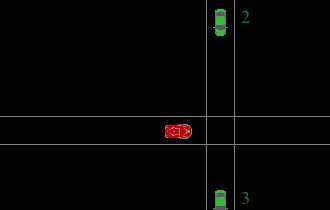
\includegraphics[width=0.99\textwidth]{figures/dqn collision example/dqn collision_1.jpeg}
		% \label{fig:y equals x}
		\caption{Ego car on the horizontal lane taking the yield action waiting for an opportunity to cross.}
\end{subfigure}%
	~ 
	\begin{subfigure}[t]{0.48\columnwidth}
		\centering
		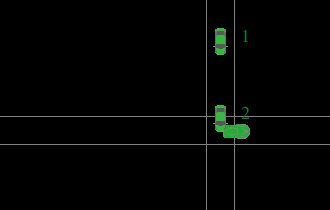
\includegraphics[width=0.99\textwidth]{figures/dqn collision example/dqn collision_3.jpeg}
		% \label{fig:double_intersection}
		\caption{Ego taking the take way action and colliding with another car on the vertical lane.}
	\end{subfigure}

	\caption{Example scenario of an Oracle DQN agent trying to drive through a gap between cars. The agent is on the horizontal lane and is red when choosing the yield action and green when choosing the take way action.}
	\label{fig:dqn_collision}
\end{figure}
% \begin{figure}[h]
%     \begin{subfigure}[b]{0.24\textwidth}
%          \centering
%          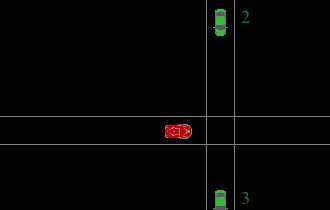
\includegraphics[width=0.99\textwidth]{figures/dqn collision example/dqn collision_1.jpeg}
%          \caption{Ego car on the horizontal lane taking the yield action waiting for an opportunity to cross.}
%          % \label{fig:y equals x}
%     \end{subfigure}
%     \hfill
%     \begin{subfigure}[b]{0.24\textwidth}
%      \centering
%      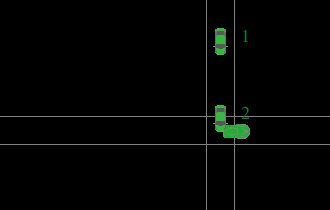
\includegraphics[width=0.99\textwidth]{figures/dqn collision example/dqn collision_3.jpeg}
%      \caption{Ego taking the take way action and colliding with another car on the vertical lane.}
%      % \label{fig:screenshot3}
%     \end{subfigure}
%     \centering
%     \caption{Example scenario of an Oracle DQN agent trying to drive through a gap between cars. The agent is on the horizontal lane and is red when choosing the yield action and green when choosing the take way action.}
%     \label{fig:dqn_collision}
% \end{figure}

The results from the previous experiment gave us a sense of the lower limit of a \gls{dqn} when not considering the intention state $\zeta$. To give a sense of an upper limit, we trained a \gls{dqn} agent on the true state \eqref{eq:state}, this is refereed to as the Oracle \gls{dqn}. 
% so to give a sense of an upper limit, a \gls{dqn} agent can perform when trained with $\zeta$. The first baseline algorithm called, oracle \gls{dqn}, is trained on the true state \eqref{eq:state}. 
% The oracle \gls{dqn} shows how well an agent could perform if it had access to the true intention $\zeta$ of other drivers during training. 
Table~\ref{tab:results_summary} shows results of the oracle \gls{dqn} and all four other agents described in Section~\ref{sec:belief_rl_algo}. 
Looking at the results, we see that even with full observability the oracle \gls{dqn} has \SI{1.05}{\percent} collisions. This shows that there are still some corner cases that the oracle \gls{dqn} agent had difficulty navigating. One such case is shown in Figure~\ref{fig:dqn_collision}, where the agent found a possible gap between cars in the picture on the left, but was hit on the tail end of ego in the figure to the right. 

\subsection{QMDP-IE and QMDP results}
\begin{figure}[!t]
    \centering
        % 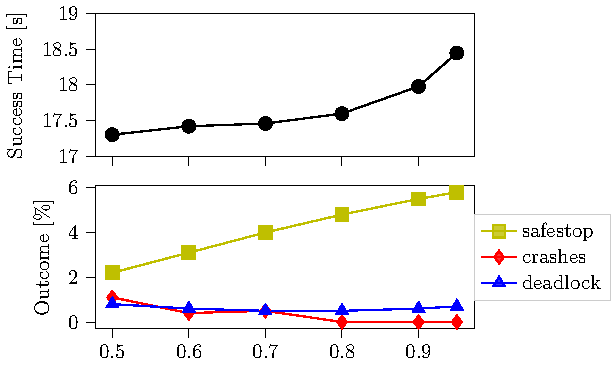
\includegraphics[width=0.99\columnwidth]{figures/figures-intention-t.pdf}
        % \include{YourThesis/papers/belief/tikz/results Intention threshold}
        % This file was created with tikzplotlib v0.10.1.
\begin{tikzpicture}

\definecolor{darkgray176}{RGB}{176,176,176}
\definecolor{goldenrod1911910}{RGB}{191,191,0}
\definecolor{green01270}{RGB}{0,127,0}
\definecolor{lightgray204}{RGB}{204,204,204}

\begin{groupplot}[group style={group size=1 by 2}]
\nextgroupplot[
height=3.5cm,
scaled x ticks=manual:{}{\pgfmathparse{#1}},
tick align=outside,
tick pos=left,
width=7cm,
x grid style={darkgray176},
xmin=-0.3, xmax=6.3,
xtick style={color=black},
xtick={0,1,2,3,4,5,6},
xticklabels={0.50,0.60,0.70,0.80,0.90,0.95,0.99},
xticklabels={},
y grid style={darkgray176},
ylabel={Success Time [s]},
ymin=14, ymax=20,
ytick style={color=black}
]
\addplot [semithick, black, mark=*, mark size=3, mark options={solid}]
table {%
0 14.9030054644809
1 15.7334844559585
2 16.1706398996236
3 16.541095890411
4 17.145
5 17.7761241291957
6 18.9131596526386
};

\nextgroupplot[
height=3.5cm,
legend cell align={left},
legend style={
  fill opacity=0.8,
  draw opacity=1,
  text opacity=1,
  at={(1,0.5)},
  anchor=west,
  draw=lightgray204
},
tick align=outside,
tick pos=left,
width=7cm,
x grid style={darkgray176},
xmin=-0.3, xmax=6.3,
xtick style={color=black},
xtick={0,1,2,3,4,5,6},
xtick={0,1,2,3,4,5,6},
xtick={0,1,2,3,4,5,6},
xtick={0,1,2,3,4,5,6},
xtick={0,1,2,3,4,5,6},
xticklabels={0.50,0.60,0.70,0.80,0.90,0.95,0.99},
xticklabels={0.50,0.60,0.70,0.80,0.90,0.95,0.99},
xticklabels={0.50,0.60,0.70,0.80,0.90,0.95,0.99},
xticklabels={0.50,0.60,0.70,0.80,0.90,0.95,0.99},
xticklabels={0.50,0.60,0.70,0.80,0.90,0.95,0.99},
y grid style={darkgray176},
ylabel={Outcome [\%]},
ymin=-1, ymax=100,
ytick style={color=black}
]
\addplot [semithick, green01270, mark=*, mark size=3, mark options={solid}]
table {%
0 73.2
1 77.2
2 79.7
3 80.3
4 80
5 78.95
6 74.85
};
\addlegendentry{goal}
\addplot [semithick, goldenrod1911910, mark=square*, mark size=3, mark options={solid}]
table {%
0 3.5
1 7.8
2 11.85
3 16.2
4 18.15
5 18.9
6 19.95
};
\addlegendentry{safestop}
\addplot [semithick, red, mark=diamond*, mark size=3, mark options={solid}]
table {%
0 23.25
1 14.95
2 8.25
3 3.3
4 1.35
5 0.95
6 0.85
};
\addlegendentry{collision}
\addplot [semithick, blue, mark=triangle*, mark size=3, mark options={solid}]
table {%
0 0.05
1 0.05
2 0.2
3 0.2
4 0.5
5 1.2
6 4.35
};
\addlegendentry{deadlock}
\end{groupplot}

% \draw ({$(current bounding box.south west)!0.5!(current bounding box.south east)$}|-{$(current bounding box.south west)!0.98!(current bounding box.north west)$}) node[
%   scale=0.5,
%   anchor=north,
%   text=black,
%   rotate=0.0
% ]{Intention threshold};
\end{tikzpicture}

        \vspace{-0.8cm}
        \caption{QMDP-IE performance (aggressiveness) for different $\zeta_\text{threshold}$ values. Increasing $\zeta_\text{threshold}$ lowers the collision rate while at the same time increasing the safe stop rate and the time it takes to reach a success state.}
    \label{fig:intent_threshold}
\end{figure}
% \discuss{This sections present the results for QMDP-IE, by first illustrating the success time and outcome for different $\zeta_\text{threshold}$ in~Figure~\ref{fig:intent_threshold}. Then, we describe how $\zeta_\text{threshold}$ is chosen and compare the results with the Oracle DQN and QMDP.}
Starting with QMDP-IE, we first demonstrate how the $\zeta_\text{threshold}$ is chosen and then compare its results with QMDP. Both algorithms use the same network weights as the Oracle DQN, but QMPD-IE is less computational than QMDP since the threshold $\zeta_\text{threshold}$ transforms the set of particles into a point estimate of the intention state, as described in Section~\ref{sec:belief_rl_algo}. Therefore, the choice of $\zeta_\text{threshold}$ is an important hyperparameter that directly correlates with the aggressiveness of the agent.

The threshold value $\zeta_\text{threshold}$, used in QMDP-IE, is determined by evaluating the agent with different $\zeta_\text{threshold}$ and observing the outcome percentage and success time. The results are shown in Figure~\ref{fig:intent_threshold}. The lowest threshold $\zeta_\text{threshold}=0.5$ is equivalent to just taking the most likely estimation of the intention and resulting in an aggressive agent. At the same time, threshold values that are too large result in a passive agent. In summary, the parameter $\zeta_\text{threshold}$ directly correlates with the agent's aggressiveness, and a good trade-off between aggressiveness and passiveness is around $\zeta_\text{threshold}=0.9$. 
With $\zeta_\text{threshold}=0.9$, QMDP-IE performs significantly better on most evaluation metrics than QMDP, see Table~\ref{tab:results_summary}. 
Moreover, QMDP-IE performs almost the same as the Oracle DQN, particularly regarding collision avoidance and success time. The method is slightly more passive than the Oracle DQN but less passive than QMDP. A feature with QMDP-IE is that the aggressiveness/passiveness can be adjusted using threshold $\zeta_\text{threshold}$ and can be changed without re-training the network weights. However, the network weights need to be trained using the true states.  

\subsection{QPF and QID results}
As opposed to QMDP-IE and QMDP, QID and QPF algorithms do not require access to the true intent during training time. While QPF trains a network using all particles, QID only uses the intention distribution from the particles, which reduces the size of the network while keeping information about the uncertainty of the intention state. 
Looking at Table~\ref{tab:results_summary}, QPF has the highest collision rate at \SI{12.15}{\percent} and the second lowest success time out of all considered algorithms, making it the most aggressive policy out of all four algorithms. 
QID collided more than QMDP-IE but still less than QMDP. This shows that training on ground truth is preferred, but QID is a good algorithm to use when ground truth data is not available. 
One downside is that QID and QPF took much longer time to train than the Oracle DQN, with up to 5 days of training. Since QID and QPF have comparable training times, this hints that the particle filter used by both algorithms is the main explanation for the computational time and that the large state space of QPF is of minor importance.


\subsection{Overtake agent}
\begin{table}[h]
\caption{Results with an overtake agent}
\label{tab:results_overtake}
\begin{tabularx}{\columnwidth}{@{}l*{10}{c}c@{}}
\toprule
Experiments & Goal reached & Safe stop & Collision & Deadlock & Success time \\ 
     & $\%$ & $\%$ & $\%$ & $\%$ & s \\ 
\midrule
Oracle DQN & $89.80$ & $0.15$ & $10.05$ & $0.00$ & $16.01$ \\ 
\textbf{QMDP-IE} & $\textbf{94.55}$ & $\textbf{0.20}$ & $\textbf{4.60}$ & $\textbf{0.65}$ & $\textbf{16.62}$ \\ 
QMDP & $79.70$ & $10.20$ & $5.95$ & $4.15$ & $19.84$ \\ 
\textbf{QID} & $\textbf{96.89}$ & $\textbf{0.11}$ & $\textbf{2.53}$ & $\textbf{0.47}$ & $\textbf{16.38}$ \\ 
QPF & $96.15$ & $0.10$ & $3.70$ & $0.05$ & $17.62$ \\ 
\bottomrule
\end{tabularx}
\end{table}

To investigate how the algorithms perform when exposed to a behavior they are not trained for, we introduce a new scenario where the conflict car is allowed to overtake the car in front. This is done by only using the free road term \eqref{eq:idm_free} for the conflict car even when there are other cars in front. The overtake scenario aims to demonstrate how adaptable the agent is to situations outside of the training set.
All algorithms are evaluated on the new overtake scenario without any retraining. 
The performance for all four algorithms, including the Oracle DQN, is summarized in Table~\ref{tab:results_overtake}. 
The collision rate for the Oracle DQN is the highest with \SI{10.05}{\percent}, this is expected since the method is trained on intention states $\zeta_n$ outside of its training set. 

In the overtake scenario, both QID and QPF have relatively low collision rates at \SI{2.53}{\percent} and \SI{3.7}{\percent} respectively, which is lower when compared to the trained scenarios in Table~\ref{tab:results_summary}. 
While the collision rate for QMDP-IE and QMDP is \SI{4.6}{\percent} and \SI{5.95}{\percent} respectively, which is higher than what they got on the trained scenario but it is also higher than QID and QPF. This indicates that QID and QPF are better at handling some scenarios outside the training set than QMDP-IE and QMDP.
QMDP also has the highest safe stop and deadlock rate at \SI{10.2}{\percent} and \SI{4.15}{\percent}, making it the most passive policy. 

\subsection{Discussion}
\label{sec:discussion}

% \textit{Is it better to train on the full distribution of the belief or use an estimation of the intention?} 
When comparing QMDP-IE with QID, it is observed that the algorithms trained on ground truth (QMDP-IE) outperform the algorithms that were trained using the belief state (QPF) or even just an estimate of the belief distribution (QID).  

The particle filter was used to create the belief state and filter the noisy observations. Hoping the flexibility of the neural network would be able to compensate for some of the inaccuracy when estimating the distribution. The higher collision rate for the QPF compared to the Oracle DQN shows that training on the full belief state can make finding a good policy difficult. 

Figure~\ref{fig:intent_threshold} shows that the aggressiveness of the policy from QMDP-IE is correlated with $\zeta_\text{threshold}$ and by choosing a relatively high value, it could get a collision rate close to the Oracle DQN, and in this case could, to some extent, compensate for the not fully optimized particle filter. The ability to adjust the aggressiveness of the policy by changing $\zeta_\text{threshold}$ is also a strength of QMDP-IE compared to QMDP and our previous black box methods that use an \gls{lstm} to estimate the latent state~\cite{Tram2018}. %For QMDP and QMDP-IE, it is not unreasonable to assume that the true intention of other drivers is accessible during training. These intentions can be labeled after the fact, by looking at if the driver ended up crossing the intersection or stopping before it. 
The downside with QMDP-IE is that, in practice, they require the true intention during training, this can be obtained by either human labeling or auto labeling techniques, which can be either expensive or tedious to generate. 

The other agents' possible actions were simplified to take way or yield. These actions could be expanded to left turn, right turn, or accelerate. In the road segment leading to the intersecting point, these actions would mainly affect the velocity profile of these cars coming into the intersection and slightly limit how fast ego can accelerate after a car that has turned into its lane. Looking at the overtake scenario, we can assume that these actions would not perform worse than using an overtake agent, shown in Table~\ref{tab:results_overtake}.

% \tommy{\cite{Seong2021} using attention to better find and use important states and cars of interest.}
\section{Conclusion}
\label{sec:conclusion}
In this study, we explored the application of reinforcement learning for safe intersection navigation, emphasizing the importance of accounting for uncertainty and planning over the distribution of intentions. Specifically, we proposed two methods for representing belief over drivers' intentions using a particle-based approach and a compact parametric representation, which can manifest as a probability distribution (QID) or a point estimate (QMDP-IE).

Our proposed particle filter exhibited promising results in estimating intention probabilities.
% , although improvements potentially could be made through enhanced prediction models and increased computational resources. 
We leveraged these intention probability estimates in QMDP-IE and QID algorithms, which demonstrated superior performance compared to respective baseline approaches QMDP and QPF. QMDP-IE, in particular, offered adjustable aggressiveness post-training, yielding a collision rate close to the Oracle DQN with an optimal threshold value $\zeta_\mathrm{threshold}$.
Furthermore, QID policies collision rate was comparable to QMDP-IE for conflict scenarios. 
% However, in a scenario outside the training set with overtake agents, QID and QPF had a lower collision rate than both QMDP-IE and QMDP. 
However, in an additional experiment involving a scenario with overtaking maneuvers, all algorithms exhibited higher collision rates compared to the standard scenario. Interestingly, QID and QPF demonstrated relatively lower collision rates, indicating adaptability to unforeseen behaviors, while QMDP displayed a more passive approach.
A downside to QID and QPF is that the training times were considerably longer, highlighting the computational demands of the particle filter.

Overall, our findings underline the importance of accounting for uncertain intentions in autonomous driving scenarios and highlight the effectiveness of leveraging intention prediction for informed decision-making. 
Future research could improve the computational demand from the particle filter by focusing on network structure that can better learn the intention state and compare the results with the QMDP-IE and QID. 